\section{Results analyses}
\subsection{Convergence of Simulations}
The residuals had a convergence criteria of $10^{-5}$. For all gridsl, the residuals converged before the maximum number of iterations (1000) was reached. The drag coefficient reached a steady value in all grids. Figures \ref{fig:residuals_grid_1} to \ref{fig:velocity_profile_grid_5} show the residuals, drag coefficient, and velocity profile for each grid.
\begin{table}[h]
    \centering
    \caption{Grid Convergence}
    \label{tab:grid_convergence}
    \begin{tabular}{ccc}
        \toprule
        Grid & Iterations & Drag Force \\
        \midrule
        1 & 57 & $2.51 \times 10^{-5}$ \\
        2 & 53 & $2.18 \times 10^{-5}$ \\
        3 & 51 & $2.08 \times 10^{-5}$ \\
        4 & 51 & $2.05 \times 10^{-5}$ \\
        5 & 52 & $2.03 \times 10^{-5}$ \\
        \bottomrule
    \end{tabular}
\end{table}
\begin{figure}[H]
    \centering
    \begin{minipage}{0.45\textwidth}
        \centering
        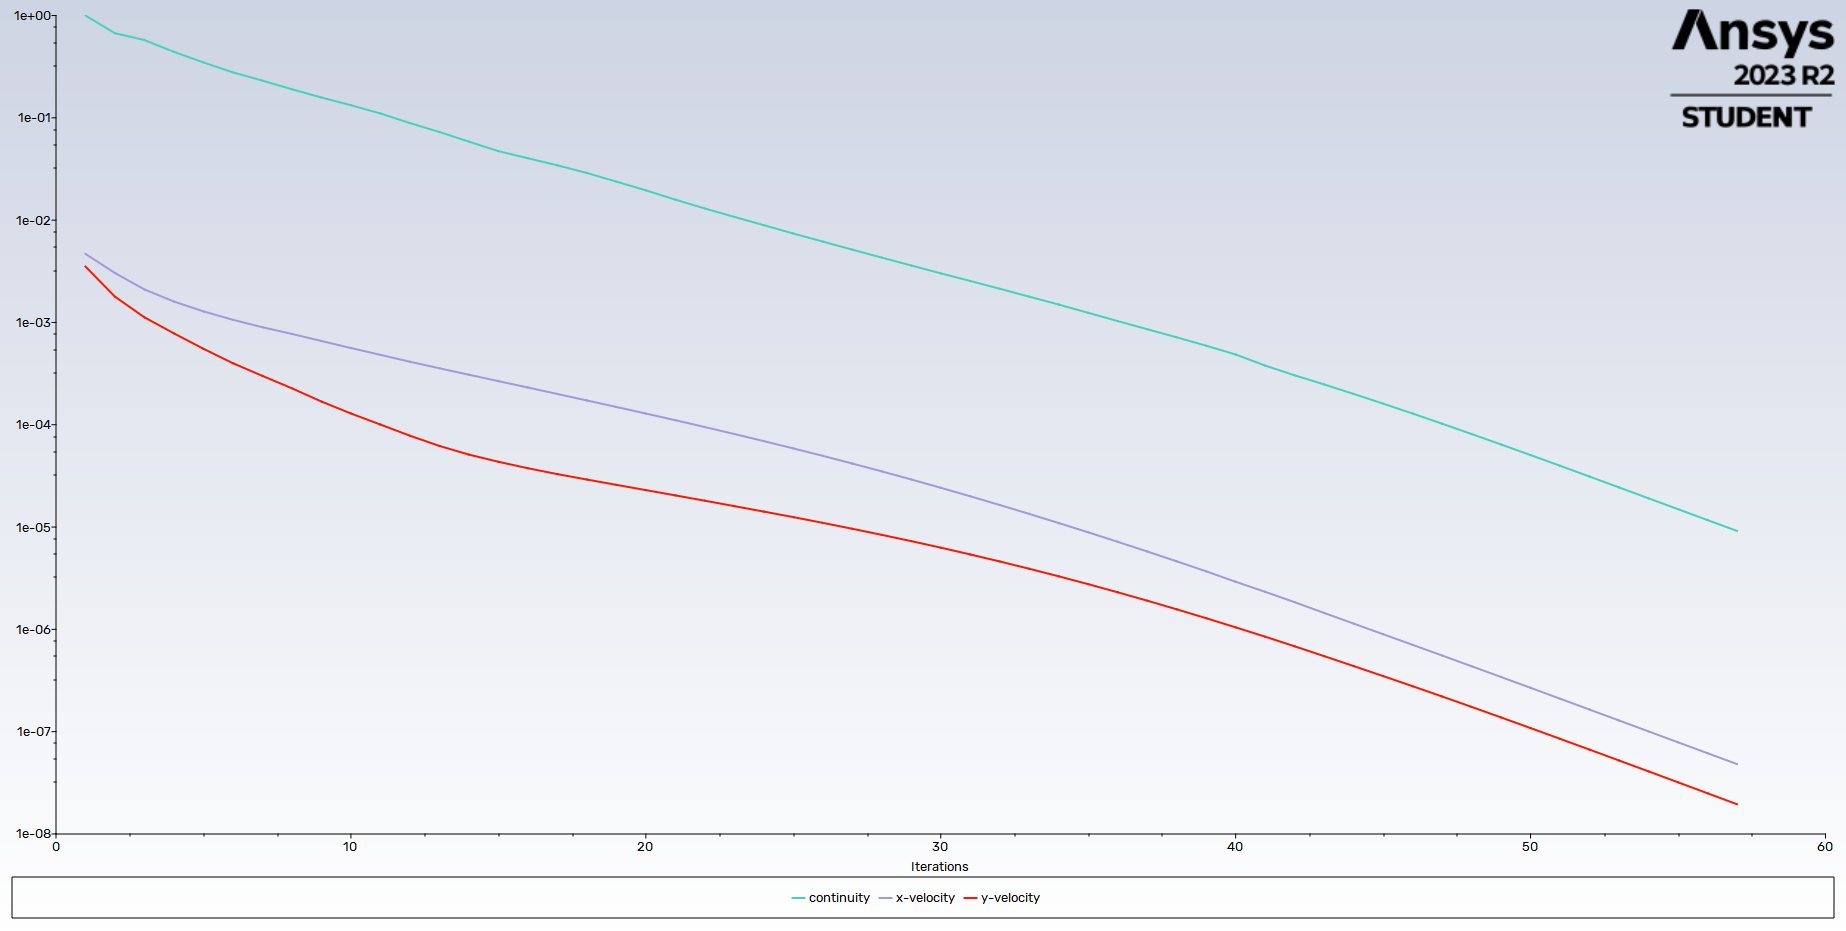
\includegraphics[width=\textwidth]{Questions/Figures/residuals grid 1.png}
        \caption{Residuals for Grid 1}
        \label{fig:residuals_grid_1}
    \end{minipage}
    \begin{minipage}{0.45\textwidth}
        \centering
        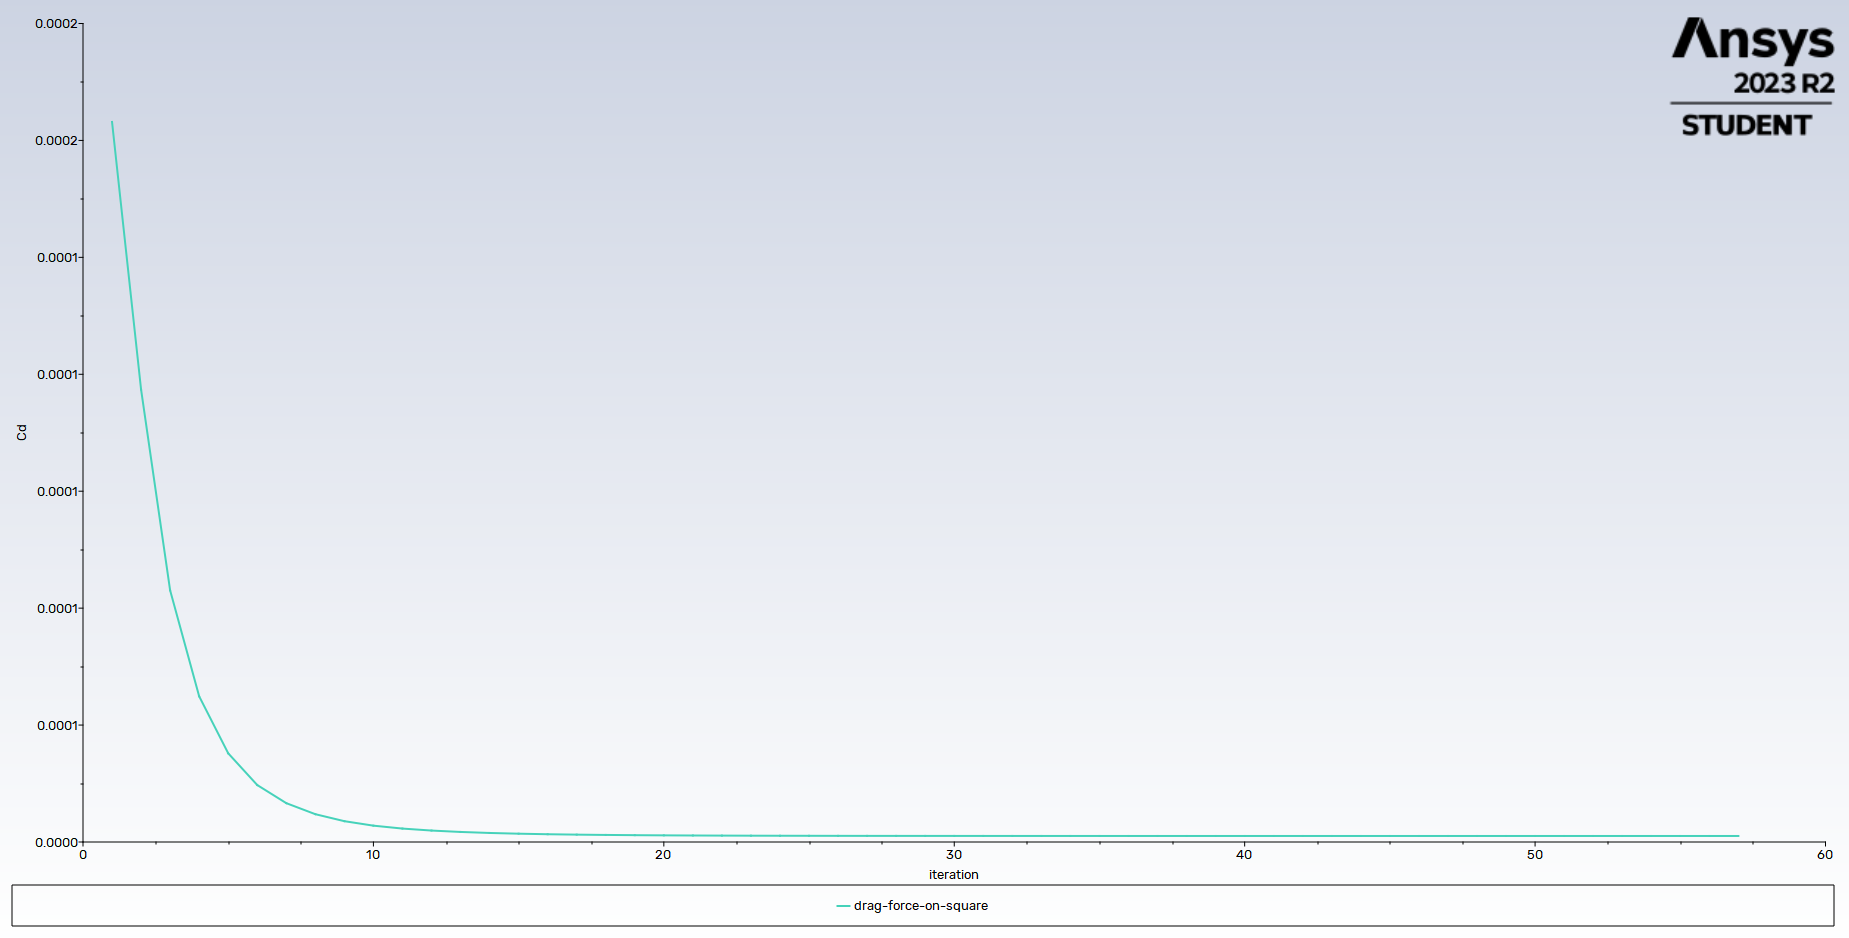
\includegraphics[width=\textwidth]{Questions/Figures/drag force on square grid 1.png}
        \caption{Drag Coefficient for Grid 1}
        \label{fig:drag_coefficient_grid_1}
    \end{minipage}
\end{figure}
\begin{figure}[H]
    \centering
    \begin{minipage}{0.45\textwidth}
        \centering
        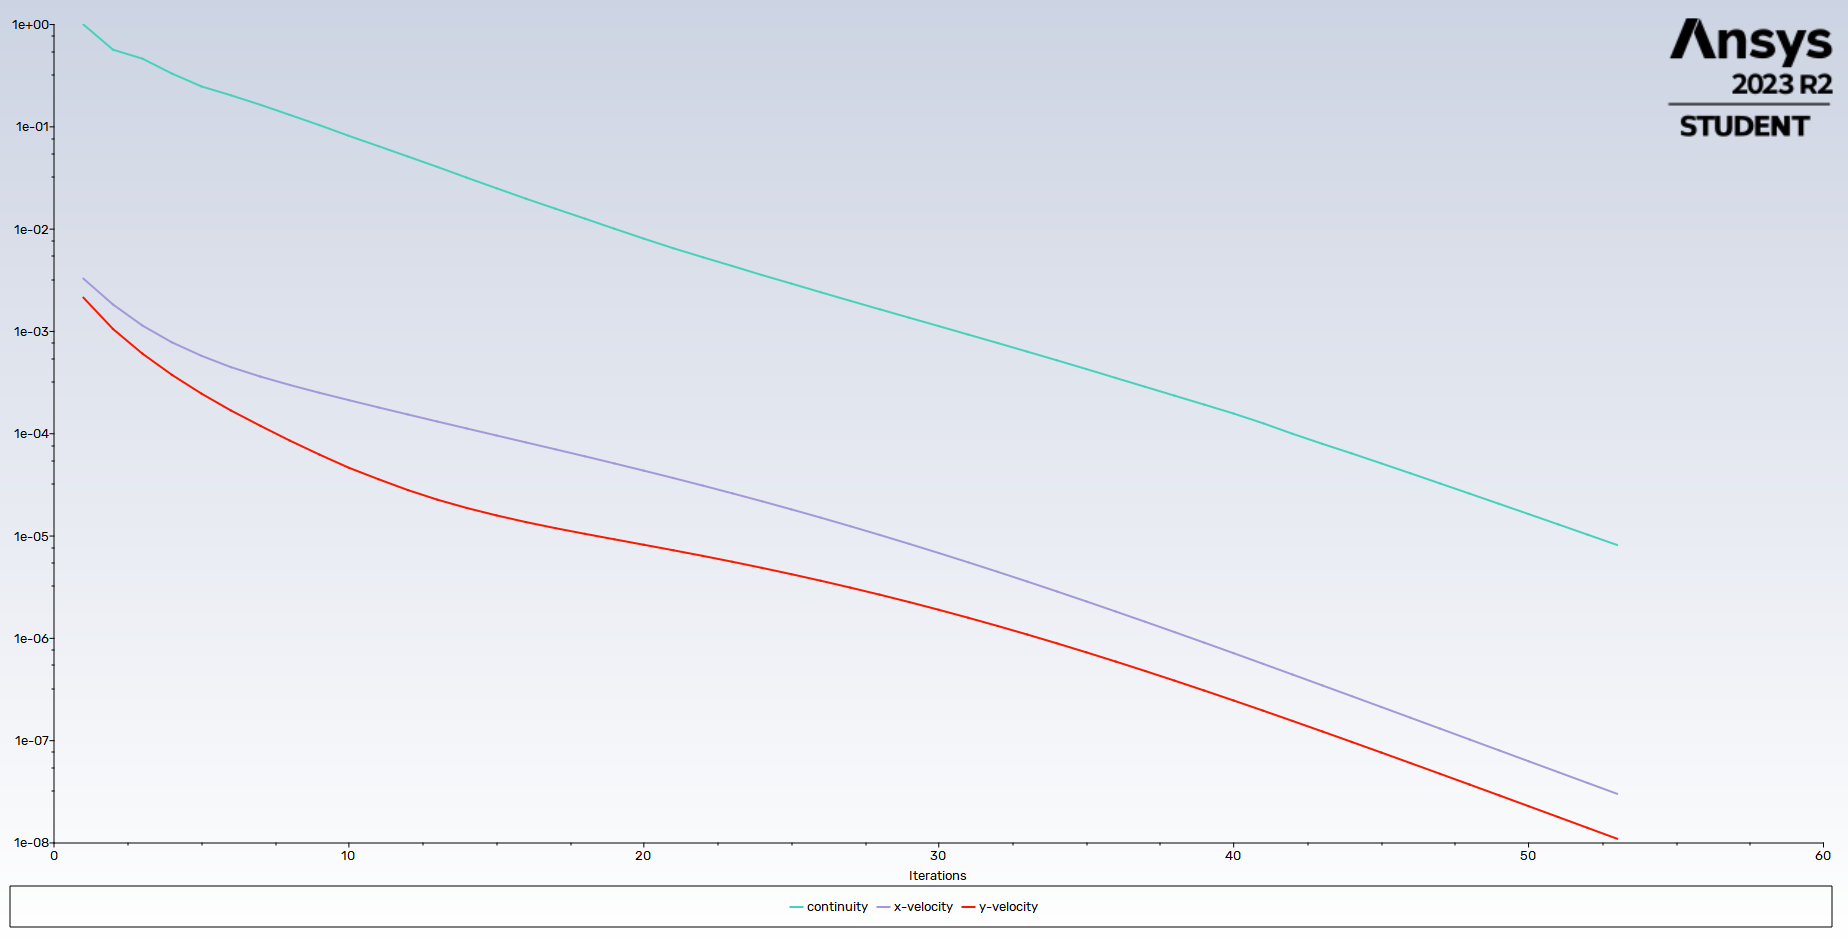
\includegraphics[width=\textwidth]{Questions/Figures/residuals grid 2.png}
        \caption{Residuals for Grid 2}
        \label{fig:residuals_grid_2}
    \end{minipage}
    \begin{minipage}{0.45\textwidth}
        \centering
        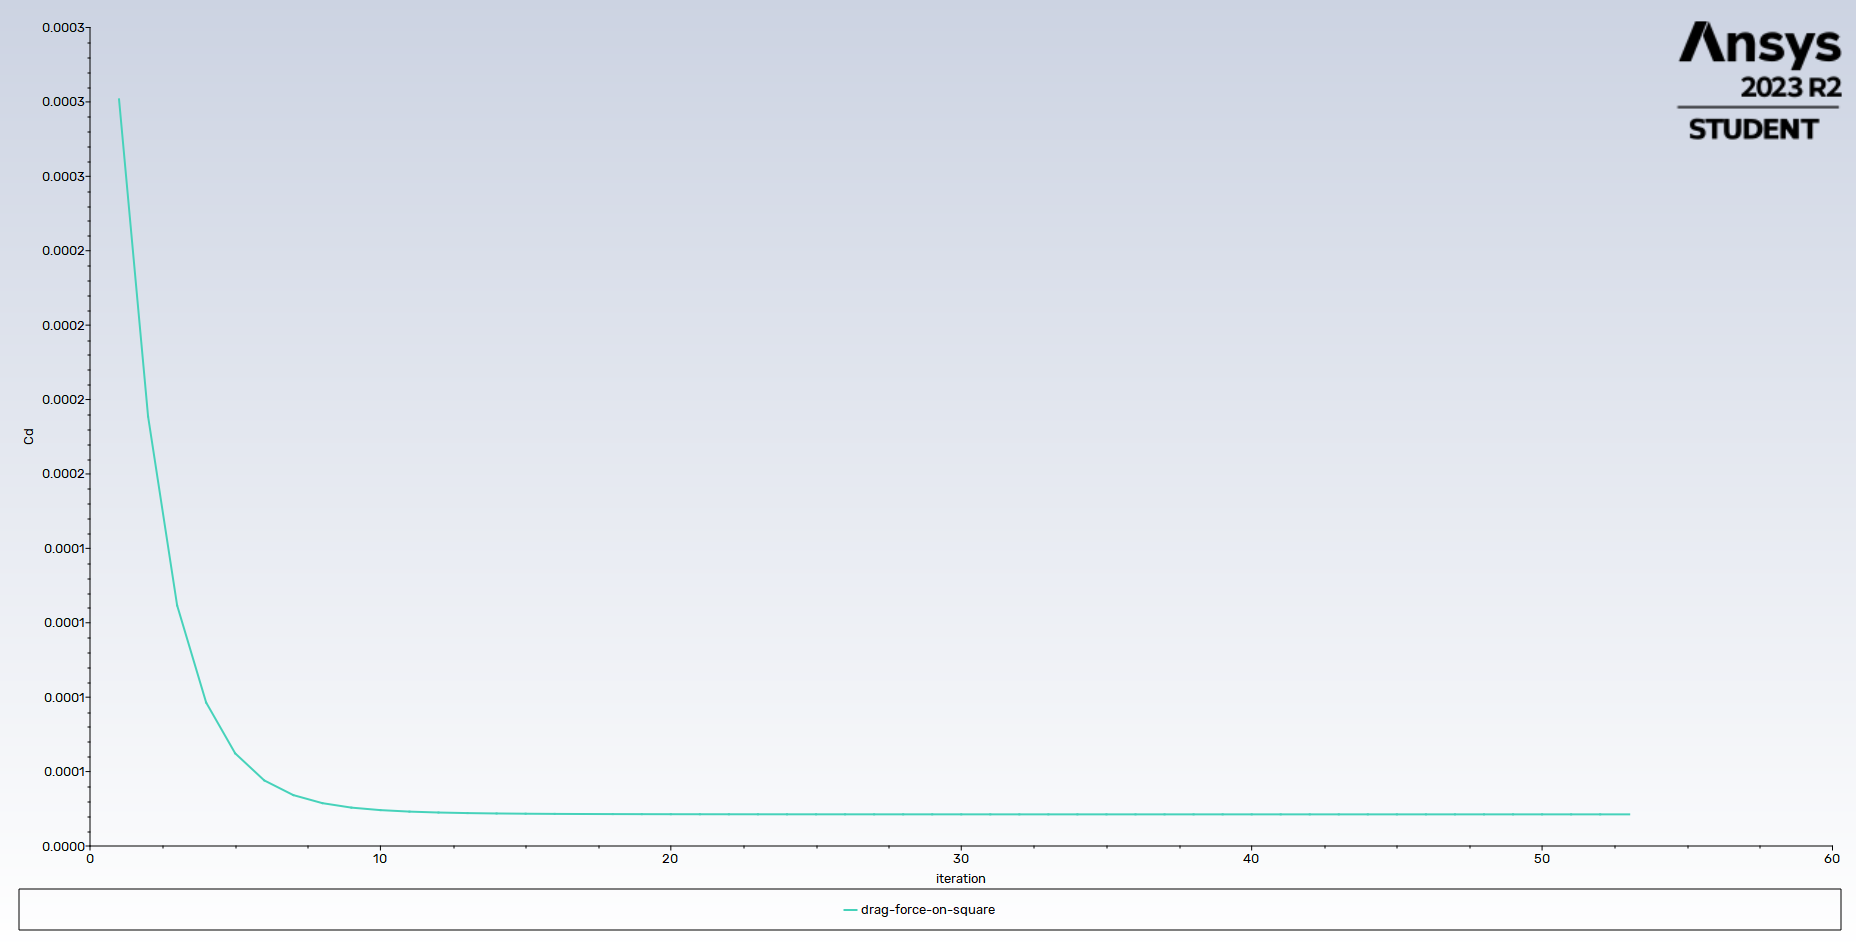
\includegraphics[width=\textwidth]{Questions/Figures/drag force on square grid 2.png}
        \caption{Drag Coefficient for Grid 2}
        \label{fig:drag_coefficient_grid_2}
    \end{minipage}
\end{figure}
\begin{figure}[H]
    \centering
    \begin{minipage}{0.45\textwidth}
        \centering
        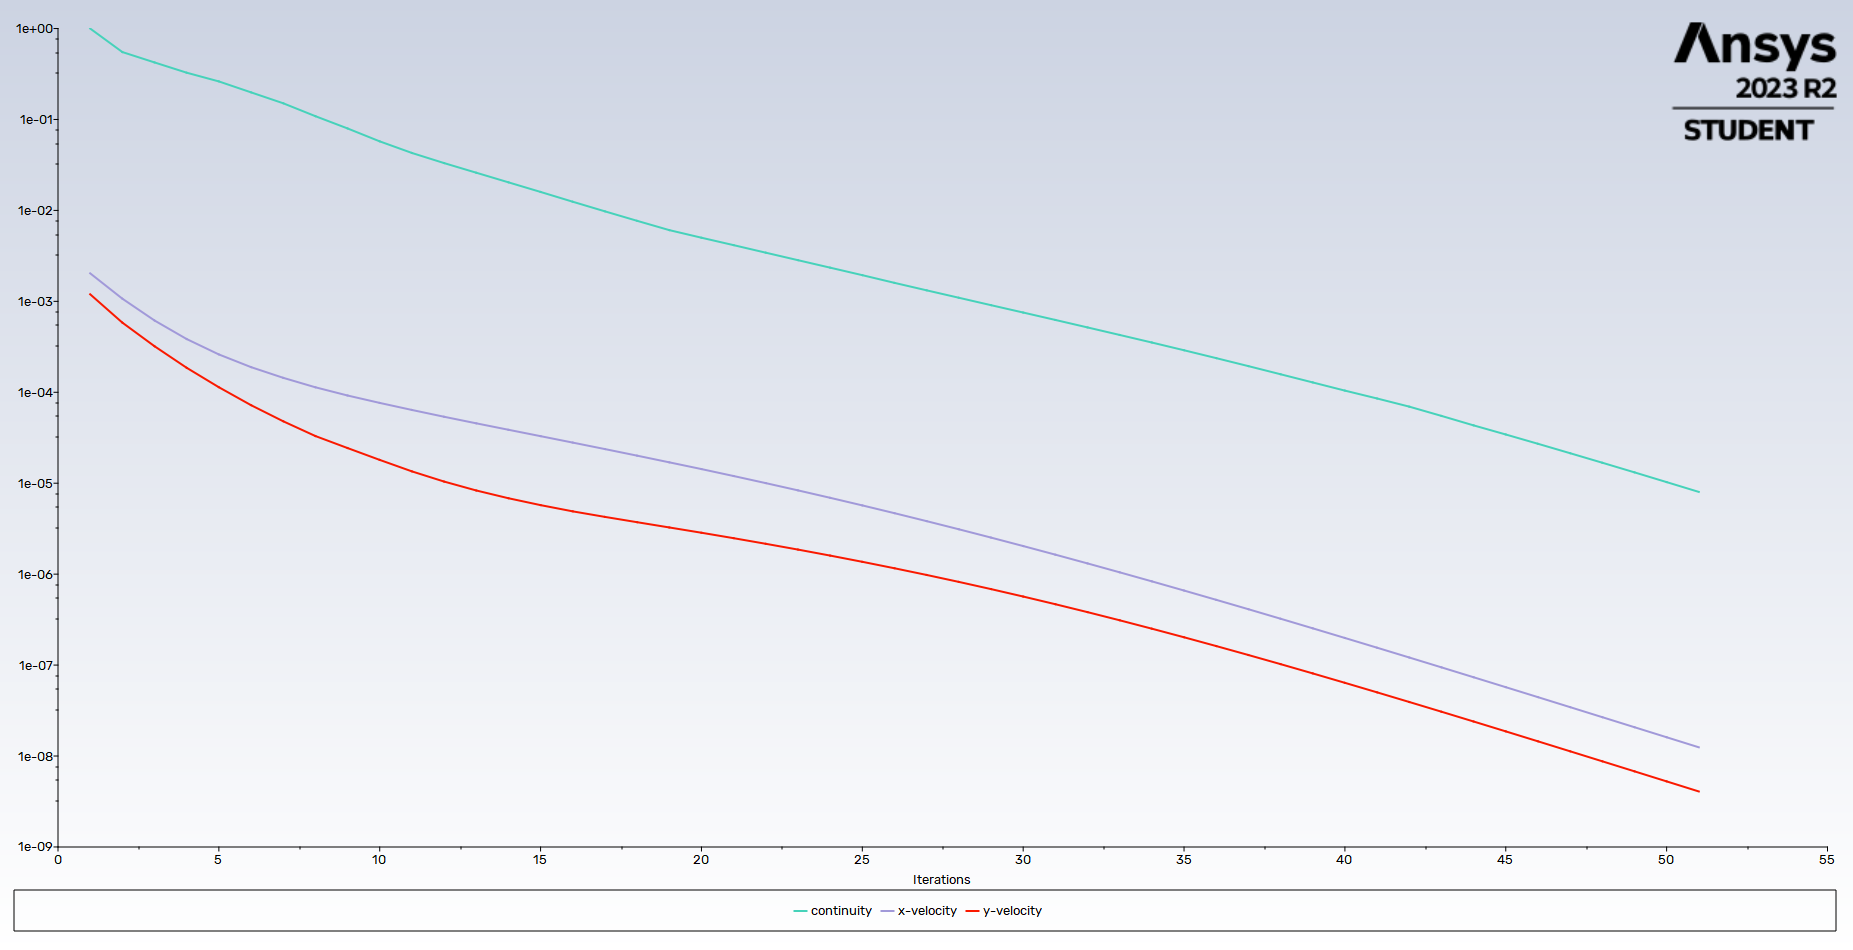
\includegraphics[width=\textwidth]{Questions/Figures/residuals grid 3.png}
        \caption{Residuals for Grid 3}
        \label{fig:residuals_grid_3}
    \end{minipage}
    \begin{minipage}{0.45\textwidth}
        \centering
        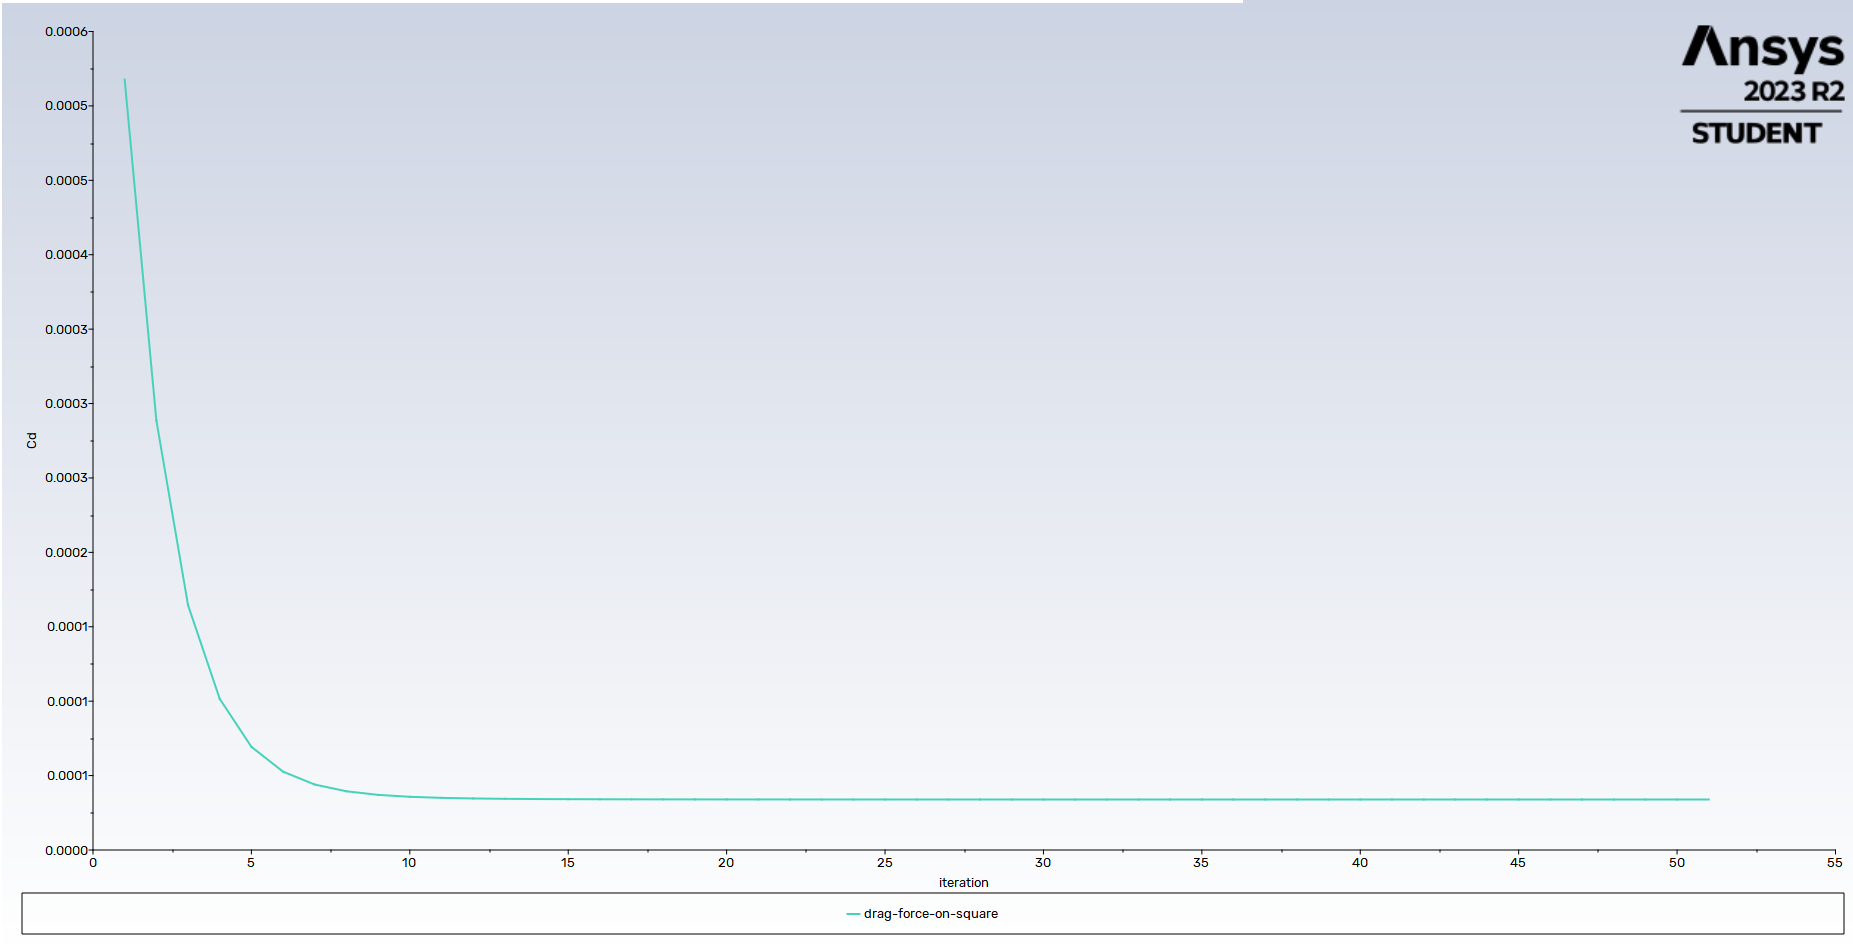
\includegraphics[width=\textwidth]{Questions/Figures/drag force on square grid 3.png}
        \caption{Drag Coefficient for Grid 3}
        \label{fig:drag_coefficient_grid_3}
    \end{minipage}
\end{figure}
\begin{figure}[H]
    \centering
    \begin{minipage}{0.45\textwidth}
        \centering
        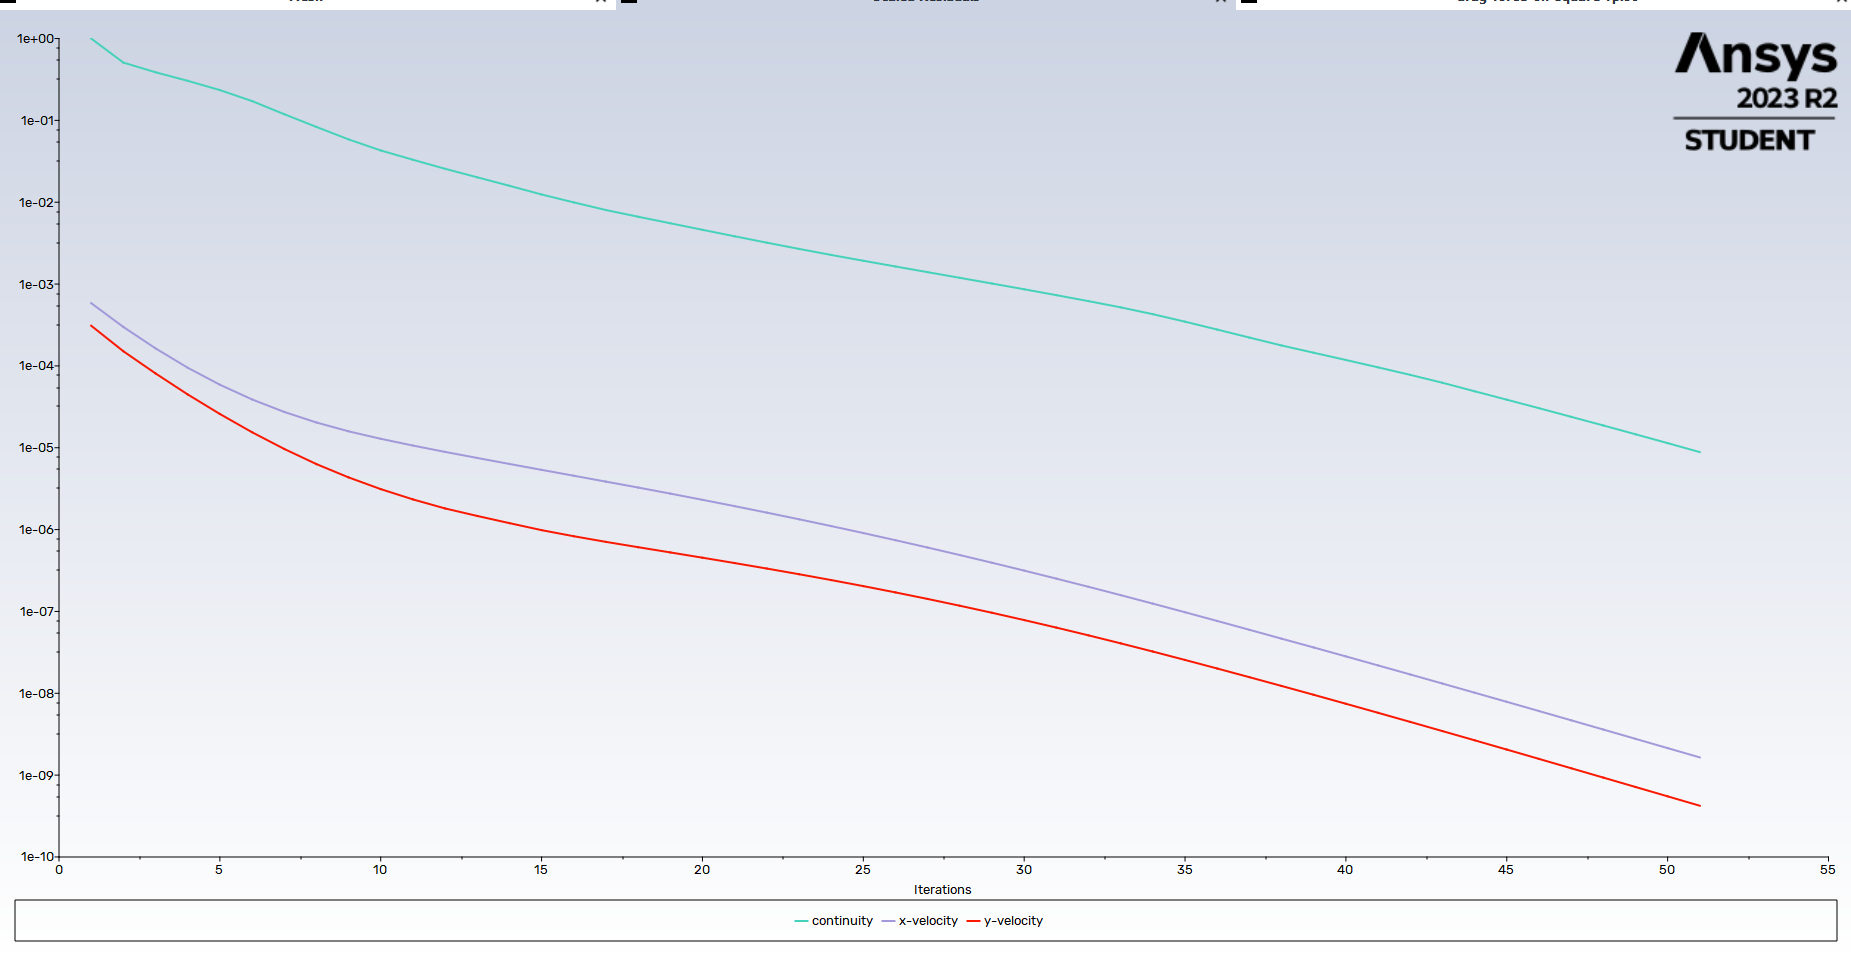
\includegraphics[width=\textwidth]{Questions/Figures/residuals grid 4.png}
        \caption{Residuals for Grid 4}
        \label{fig:residuals_grid_4}
    \end{minipage}
    \begin{minipage}{0.45\textwidth}
        \centering
        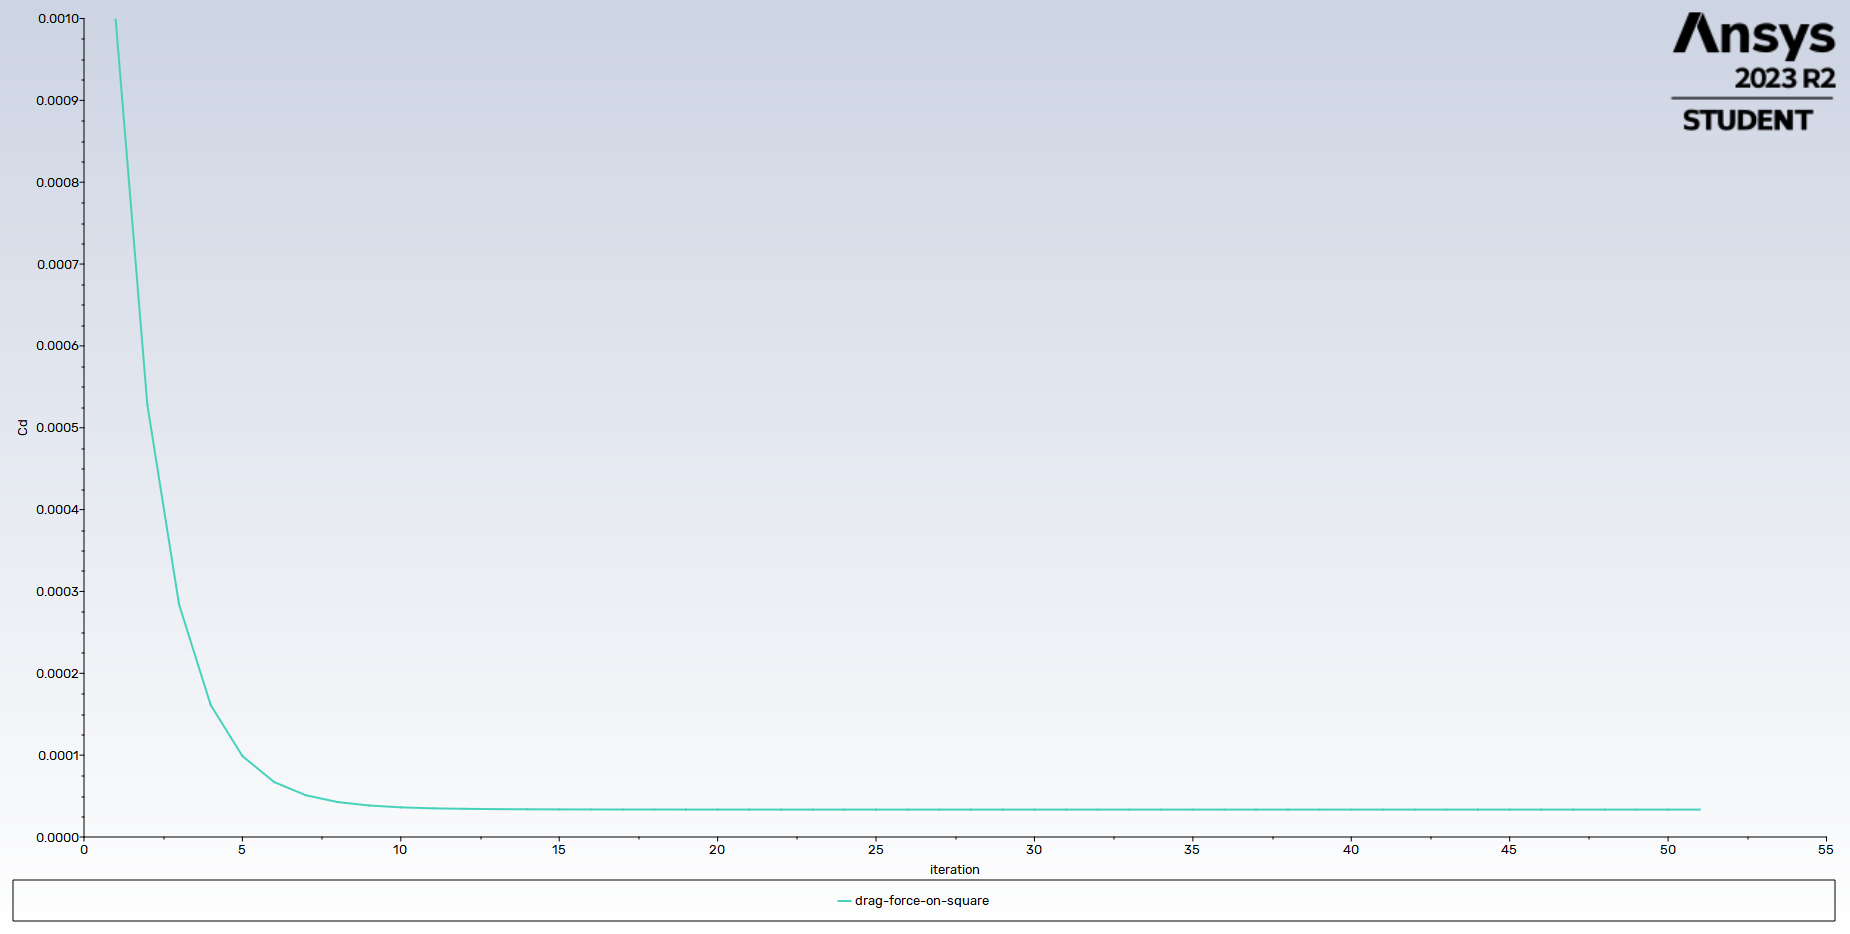
\includegraphics[width=\textwidth]{Questions/Figures/drag force on square grid 4.png}
        \caption{Drag Coefficient for Grid 4}
        \label{fig:drag_coefficient_grid_4}
    \end{minipage}
\end{figure}
\begin{figure}[H]
    \centering
    \begin{minipage}{0.45\textwidth}
        \centering
        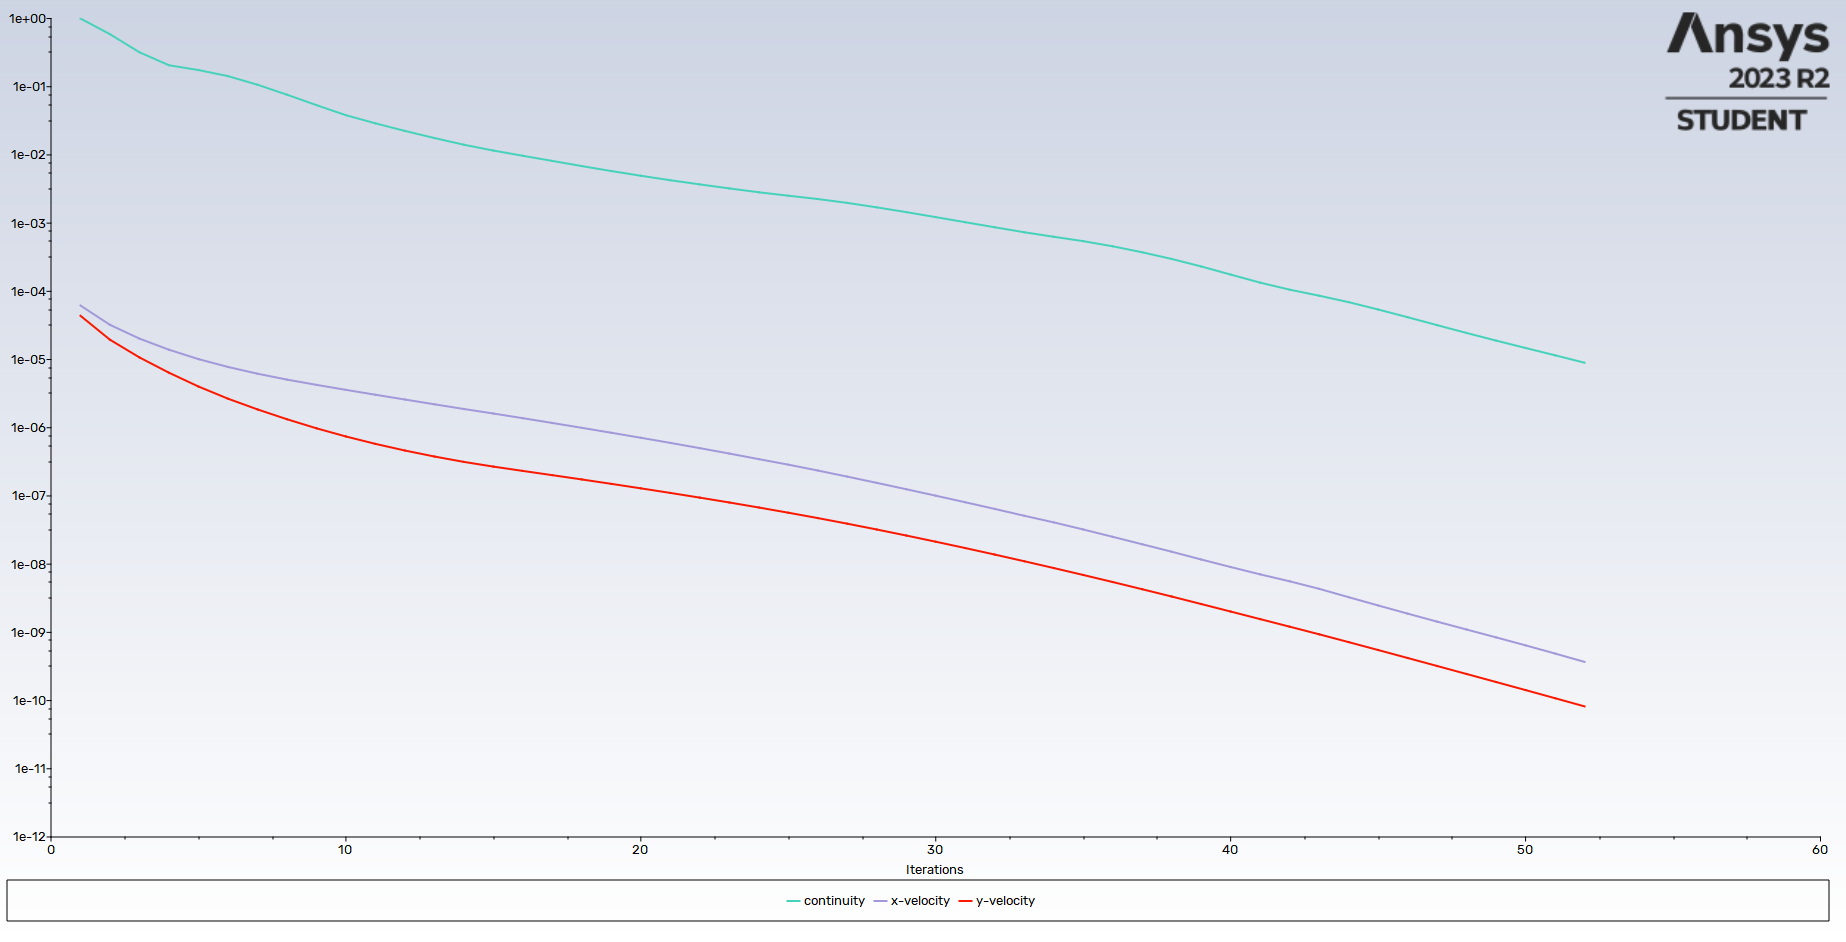
\includegraphics[width=\textwidth]{Questions/Figures/residuals grid 5.png}
        \caption{Residuals for Grid 5}
        \label{fig:residuals_grid_5}
    \end{minipage}
    \begin{minipage}{0.45\textwidth}
        \centering
        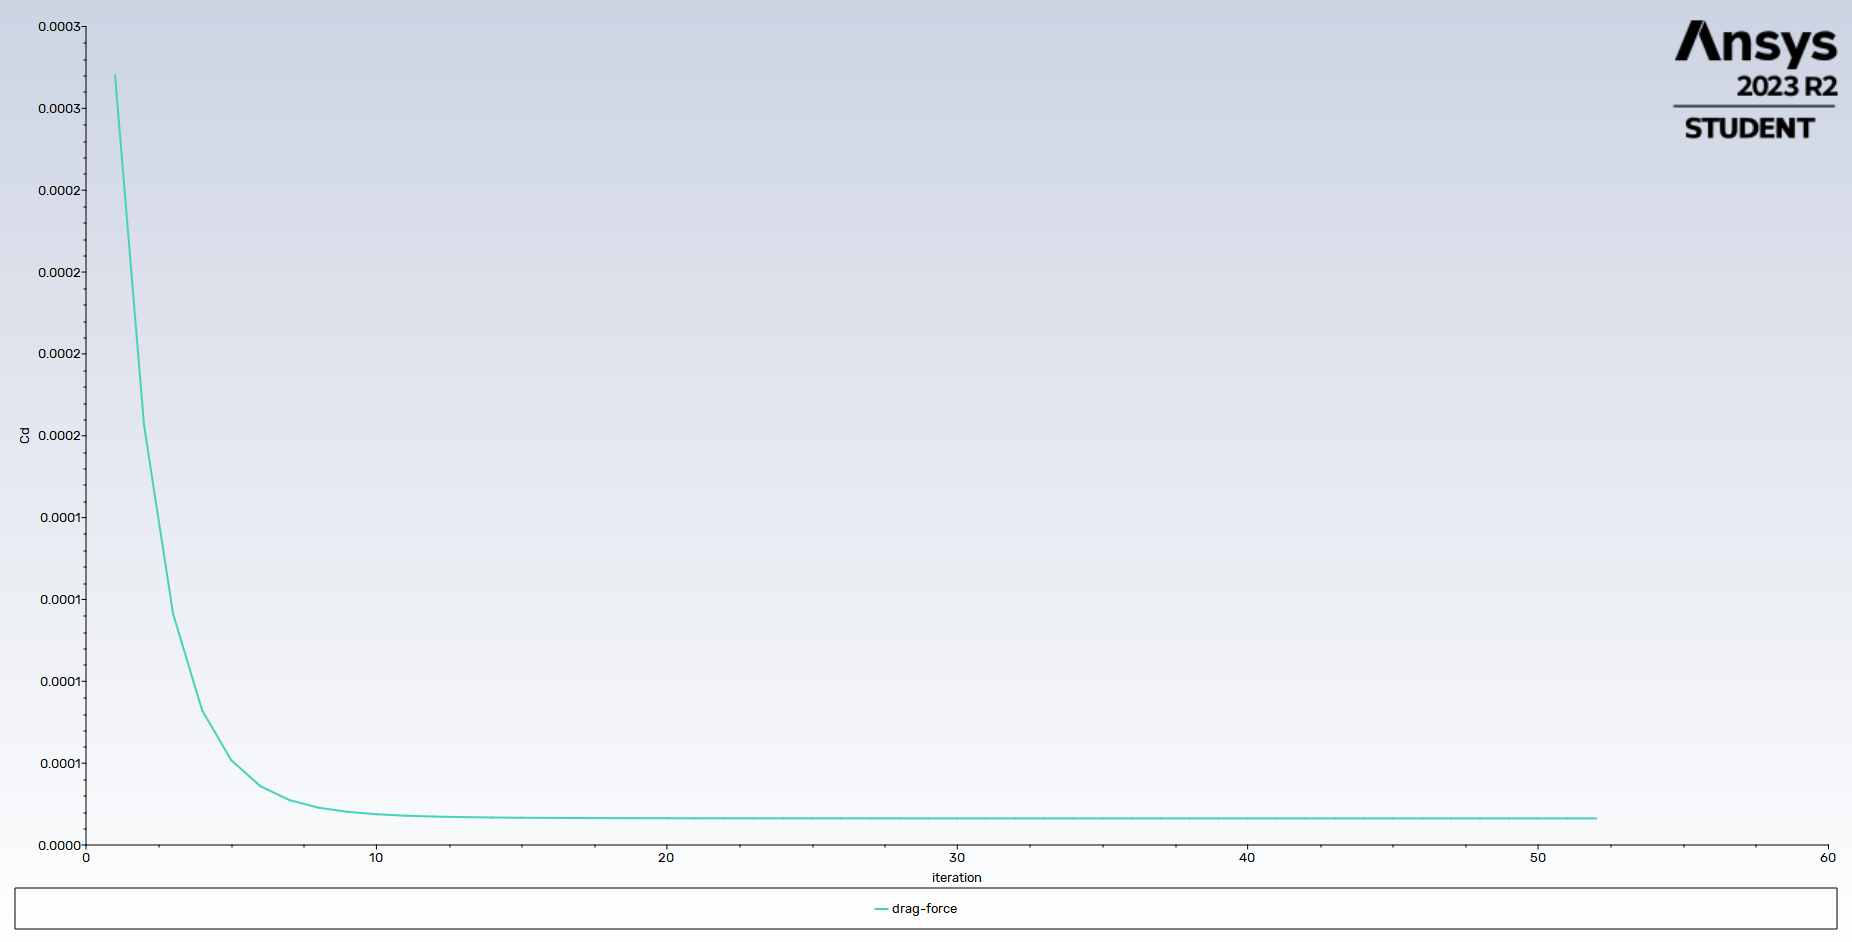
\includegraphics[width=\textwidth]{Questions/Figures/drag force on square grid 5.png}
        \caption{Drag Coefficient for Grid 5}
        \label{fig:drag_coefficient_grid_5}
    \end{minipage}
\end{figure}
\begin{figure}[H]
    \centering
    \begin{minipage}{0.45\textwidth}
        \centering
        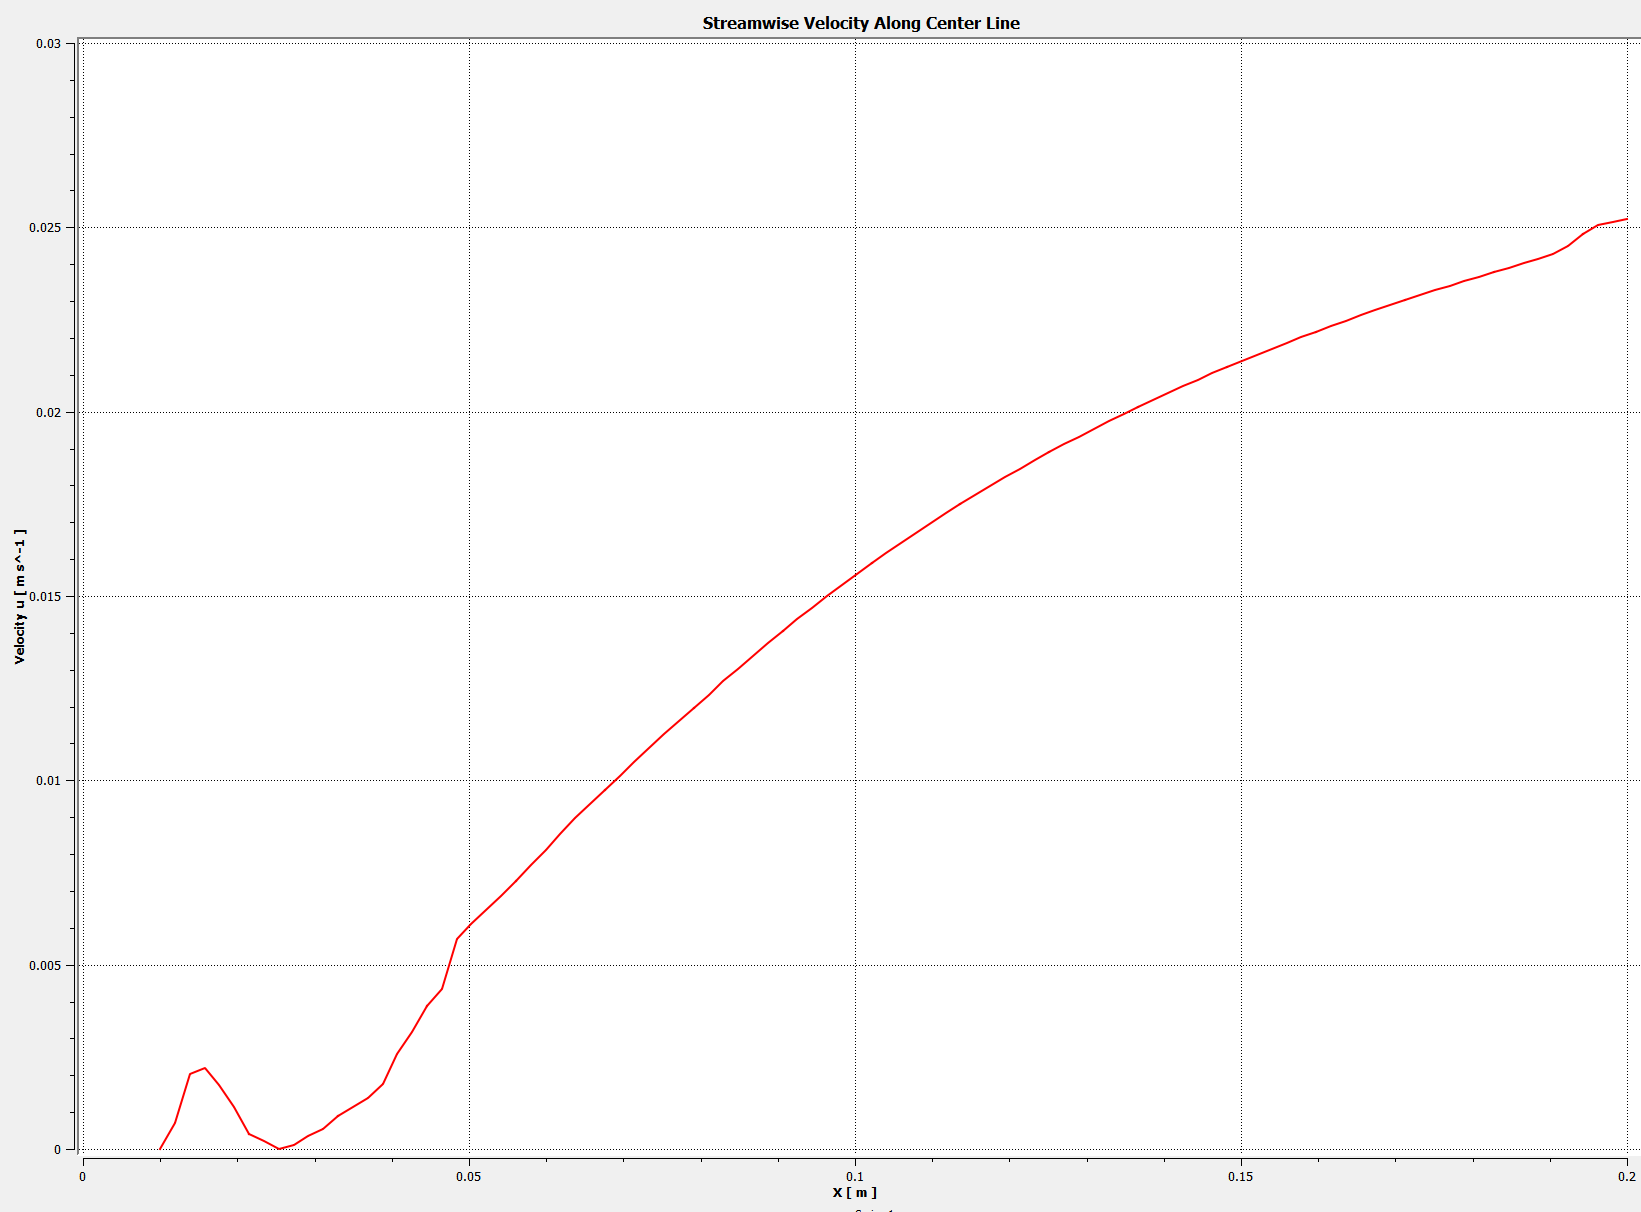
\includegraphics[width=\textwidth]{Questions/Figures/u velocity along centerline grid 1.png}
        \caption{Velocity Profile for Grid 1}
        \label{fig:velocity_profile_grid_1}
    \end{minipage}
    \begin{minipage}{0.45\textwidth}
        \centering
        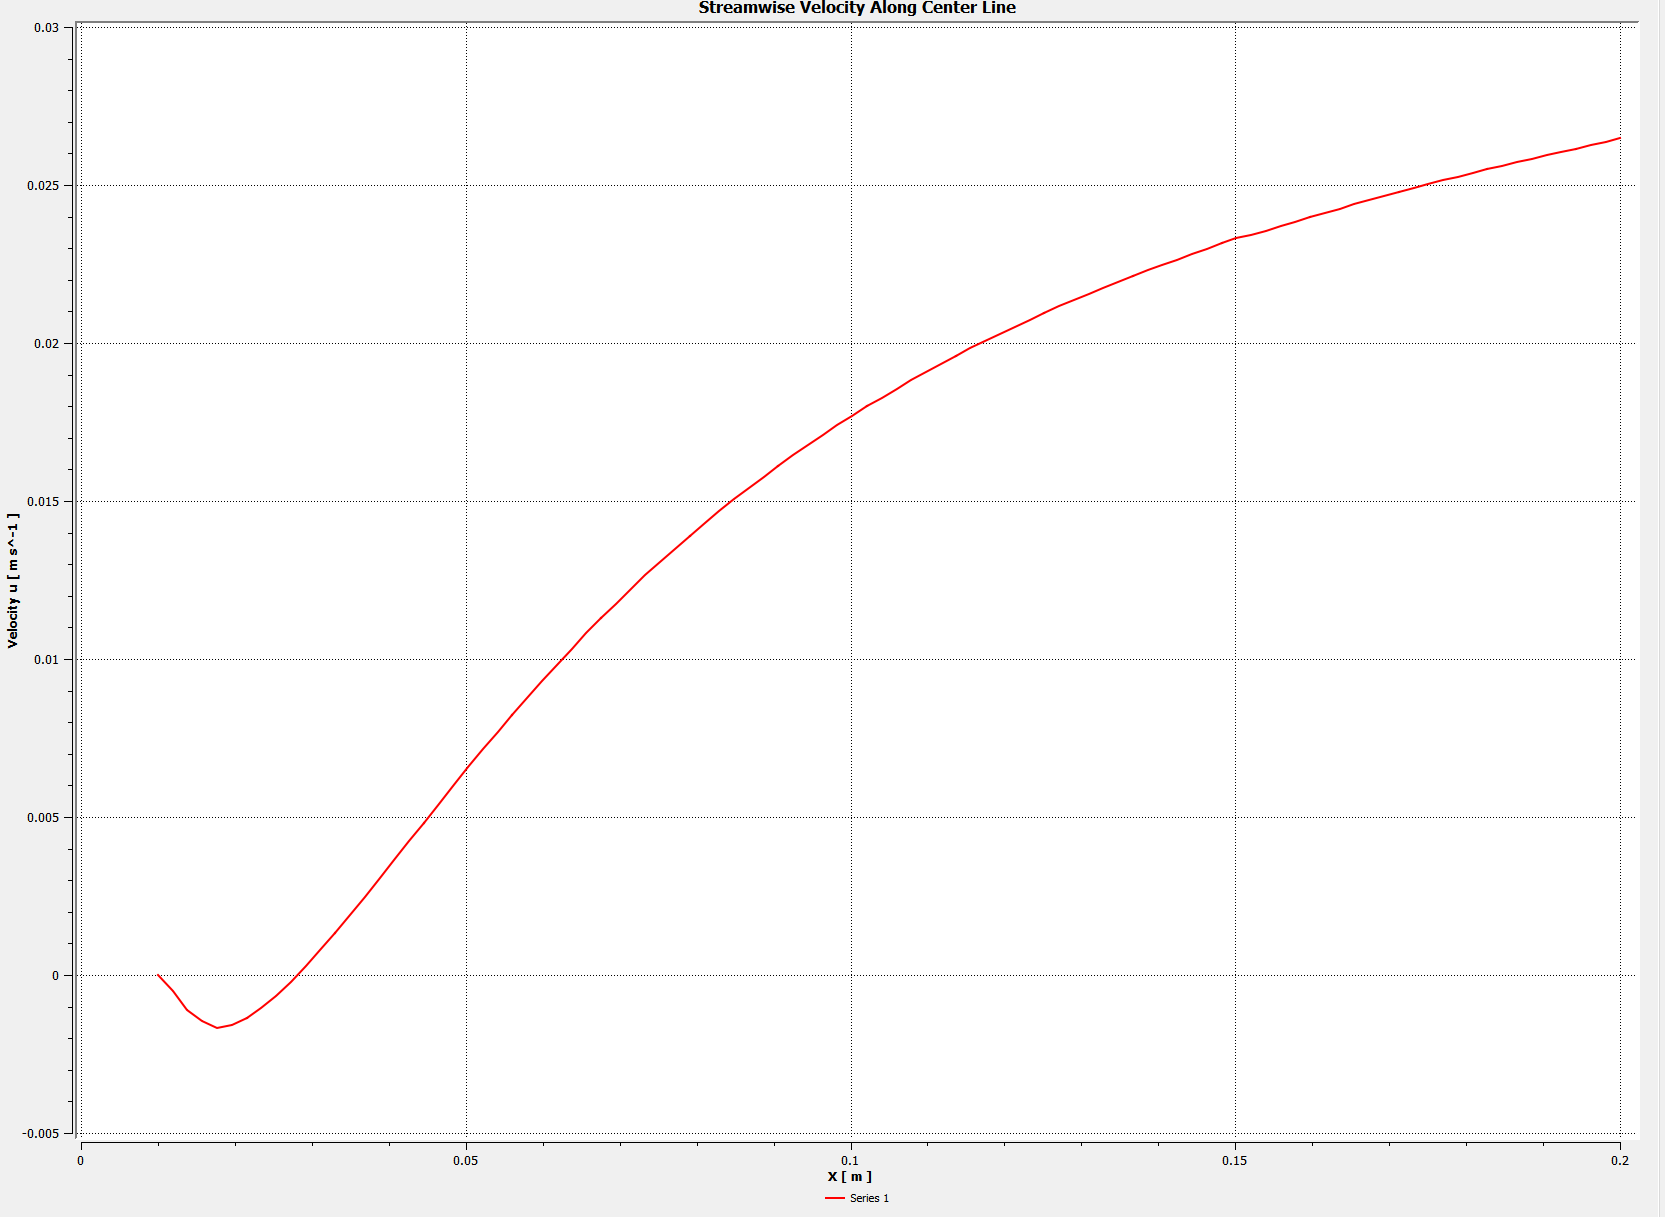
\includegraphics[width=\textwidth]{Questions/Figures/u velocity along centerline grid 2.png}
        \caption{Velocity Profile for Grid 2}
        \label{fig:velocity_profile_grid_2}
    \end{minipage}
\end{figure}
\begin{figure}[H]
    \centering
    \begin{minipage}{0.45\textwidth}
        \centering
        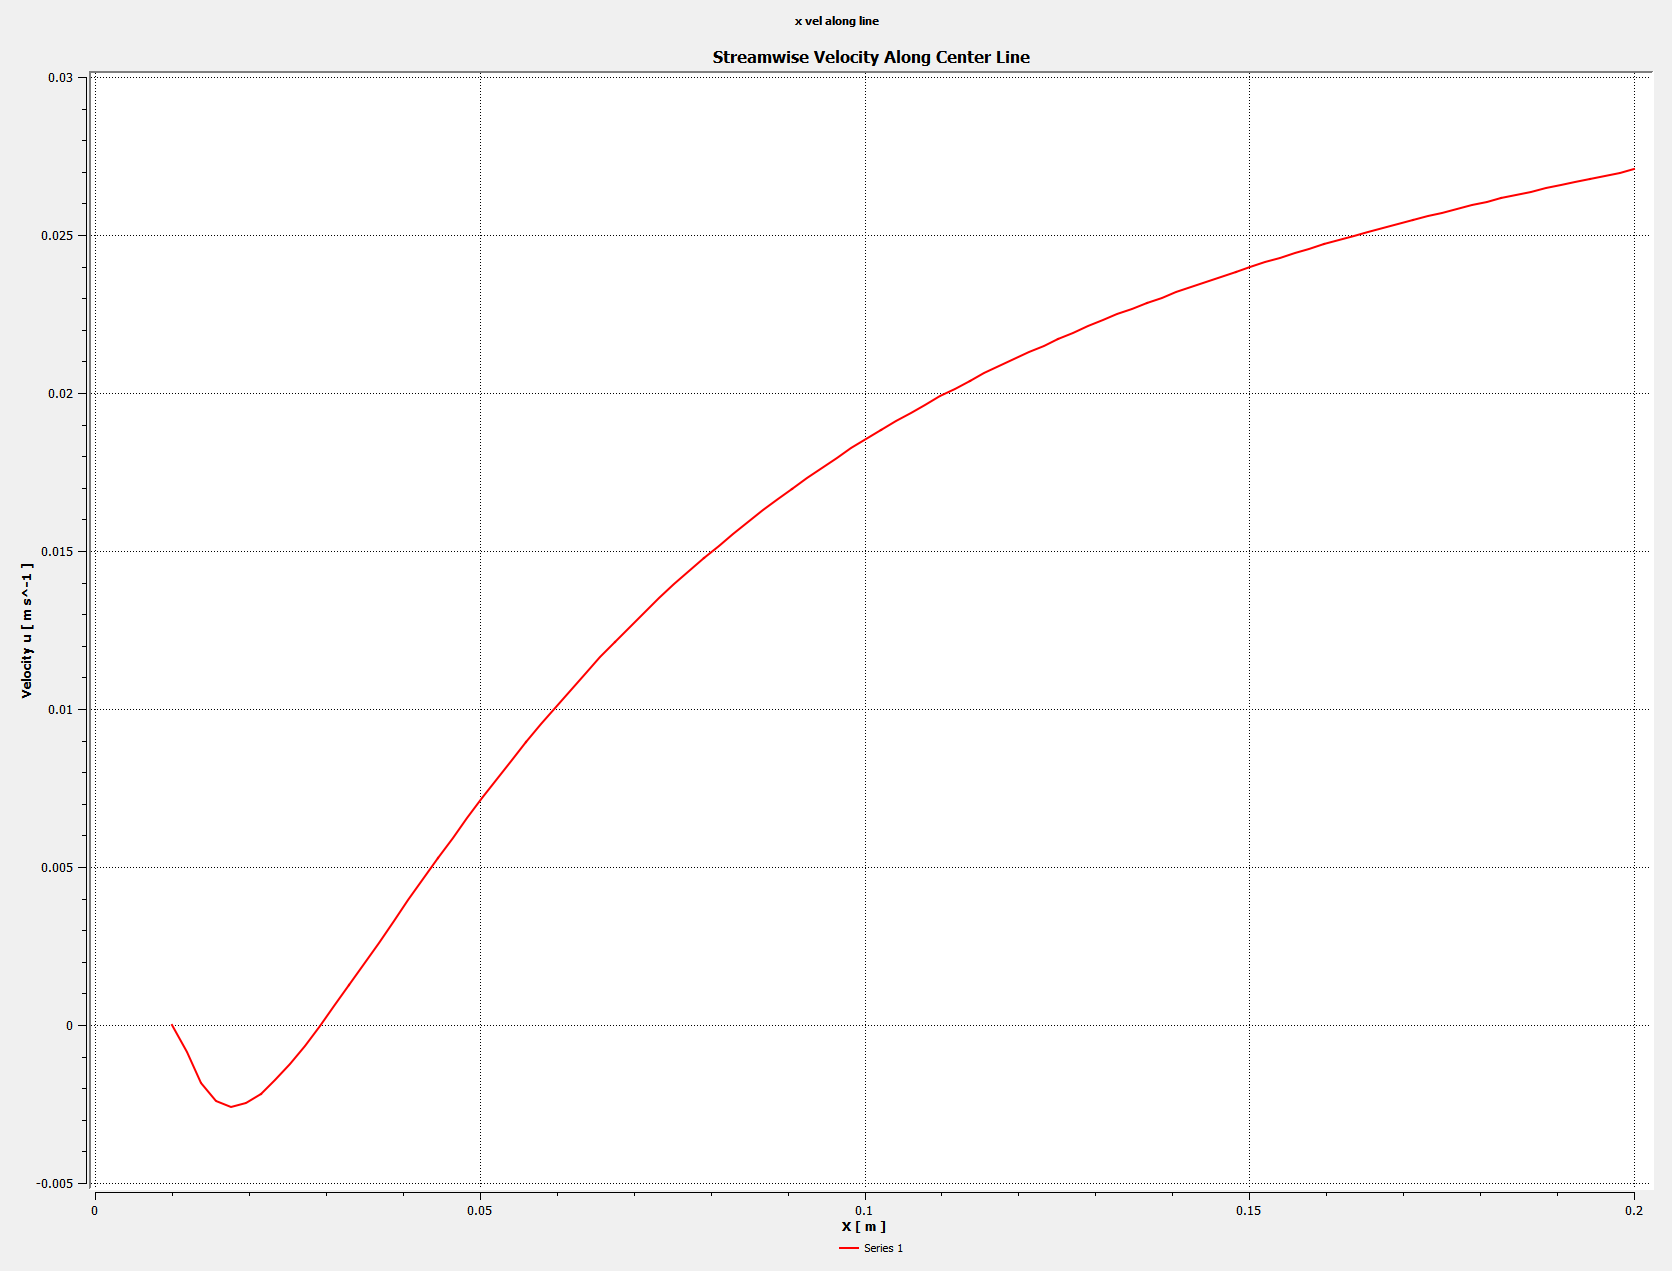
\includegraphics[width=\textwidth]{Questions/Figures/u velocity along centerline grid 3.png}
        \caption{Velocity Profile for Grid 3}
        \label{fig:velocity_profile_grid_3}
    \end{minipage}
    \begin{minipage}{0.45\textwidth}
        \centering
        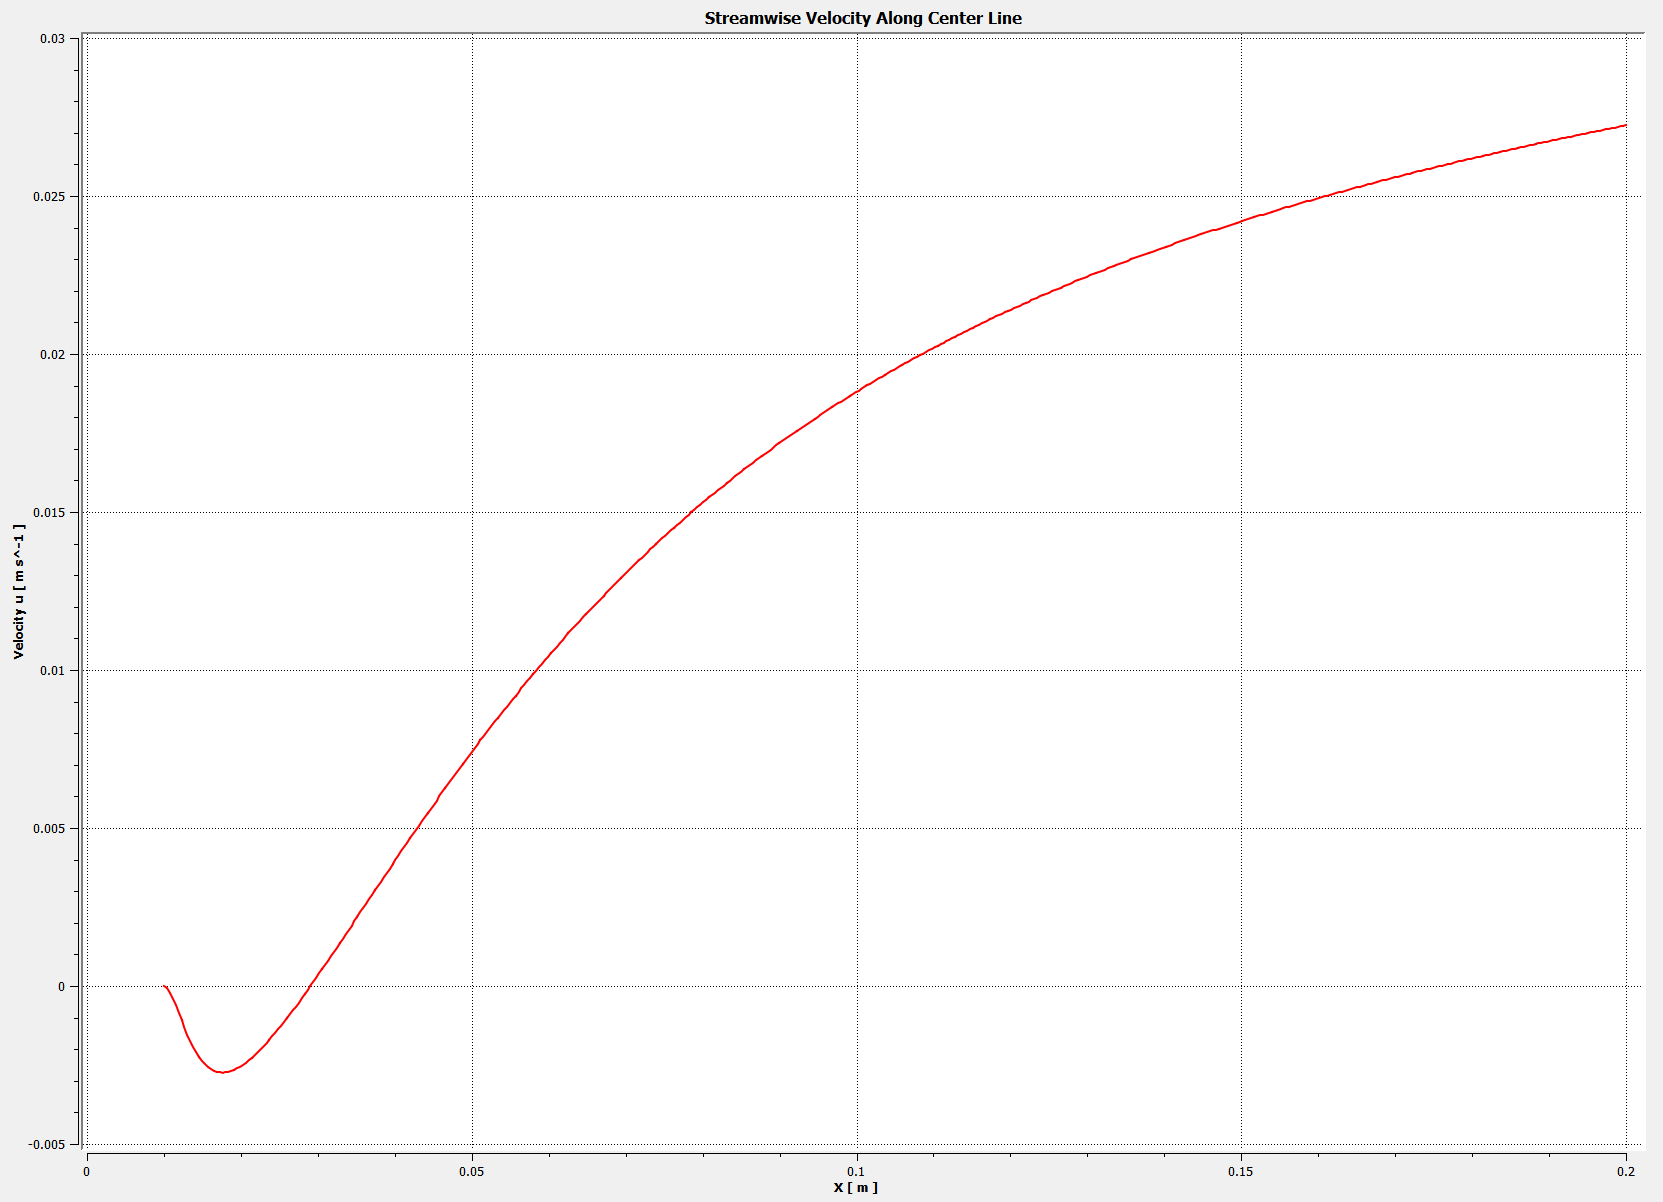
\includegraphics[width=\textwidth]{Questions/Figures/u velocity along centerline grid 4.png}
        \caption{Velocity Profile for Grid 4}
        \label{fig:velocity_profile_grid_4}
    \end{minipage}
\end{figure}
\begin{figure}[H]
    \centering
    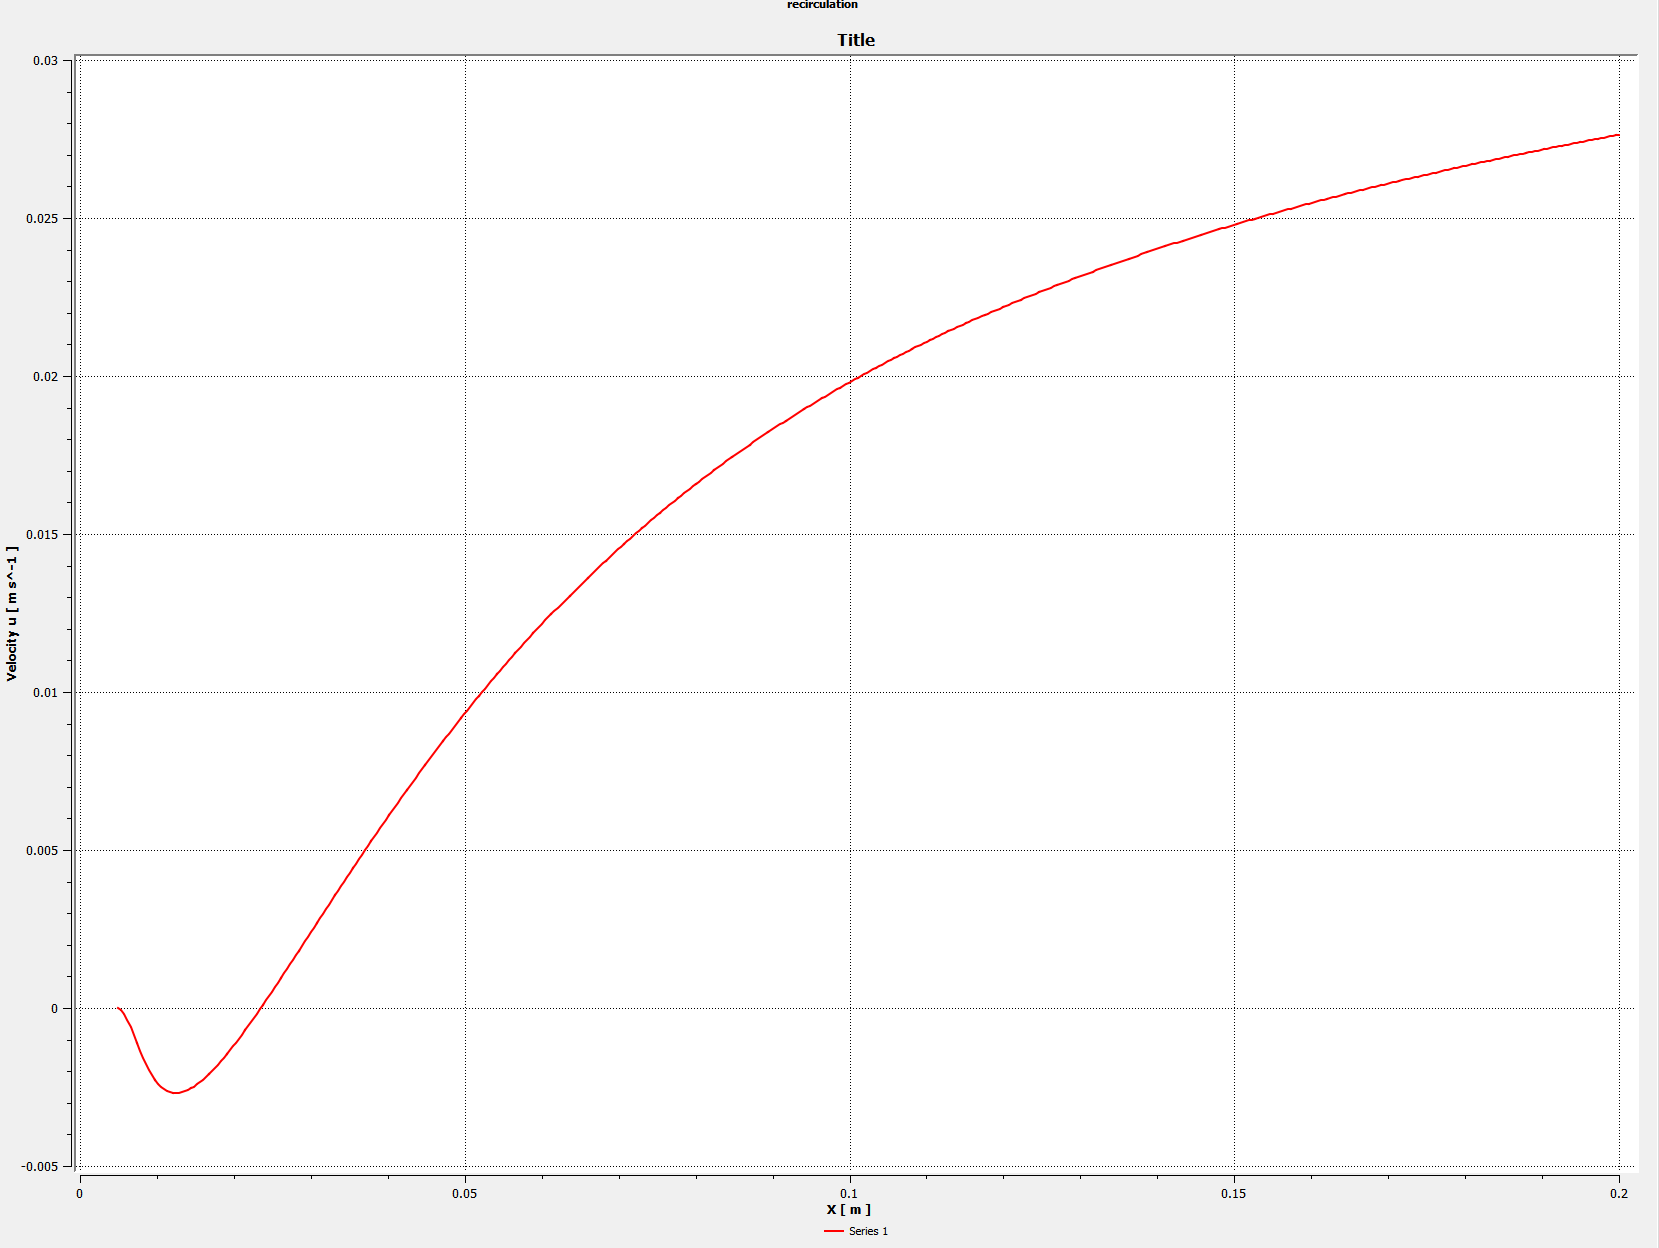
\includegraphics[width=0.45\textwidth]{Questions/Figures/u velocity along centerline grid 5.png}
    \caption{Velocity Profile for Grid 5}
    \label{fig:velocity_profile_grid_5}
\end{figure}

\subsection{Analyses of the Velocity Fields}
The contours are shown in Figures \ref{fig:velocity_contour_grid_1} and \ref{fig:velocity_contour_grid_5}. The flow is symmetric about the centerline. The flow behind the square object is observable in grid 1, but much more refined in grid 5. In grid 5, two flanges of high velocity flow can be seen to the side of the square object. In comparison, the whole region to the side of the square object is a high velocity region in grid 1, which makes less physical sense. Grid 5 should be used since the results are more physical.

The streamlines are shown in Figures \ref{fig:streamlines_grid_1}, \ref{fig:streamlines_grid_3}, and \ref{fig:streamlines_grid_5}. Again, the flow is symmetric about the centerline. A small vortex region can be seen from behind the square object in grids 3 and 5. The flow aspects are difficult to discern in grid 1. Considering that meshing grid 5 took roughly 20 minutes to mesh on my desktop computer, grid 3 is a good compromise between accuracy and computational cost.

\begin{figure}[H]
    \centering
    \begin{minipage}{0.45\textwidth}
        \centering
        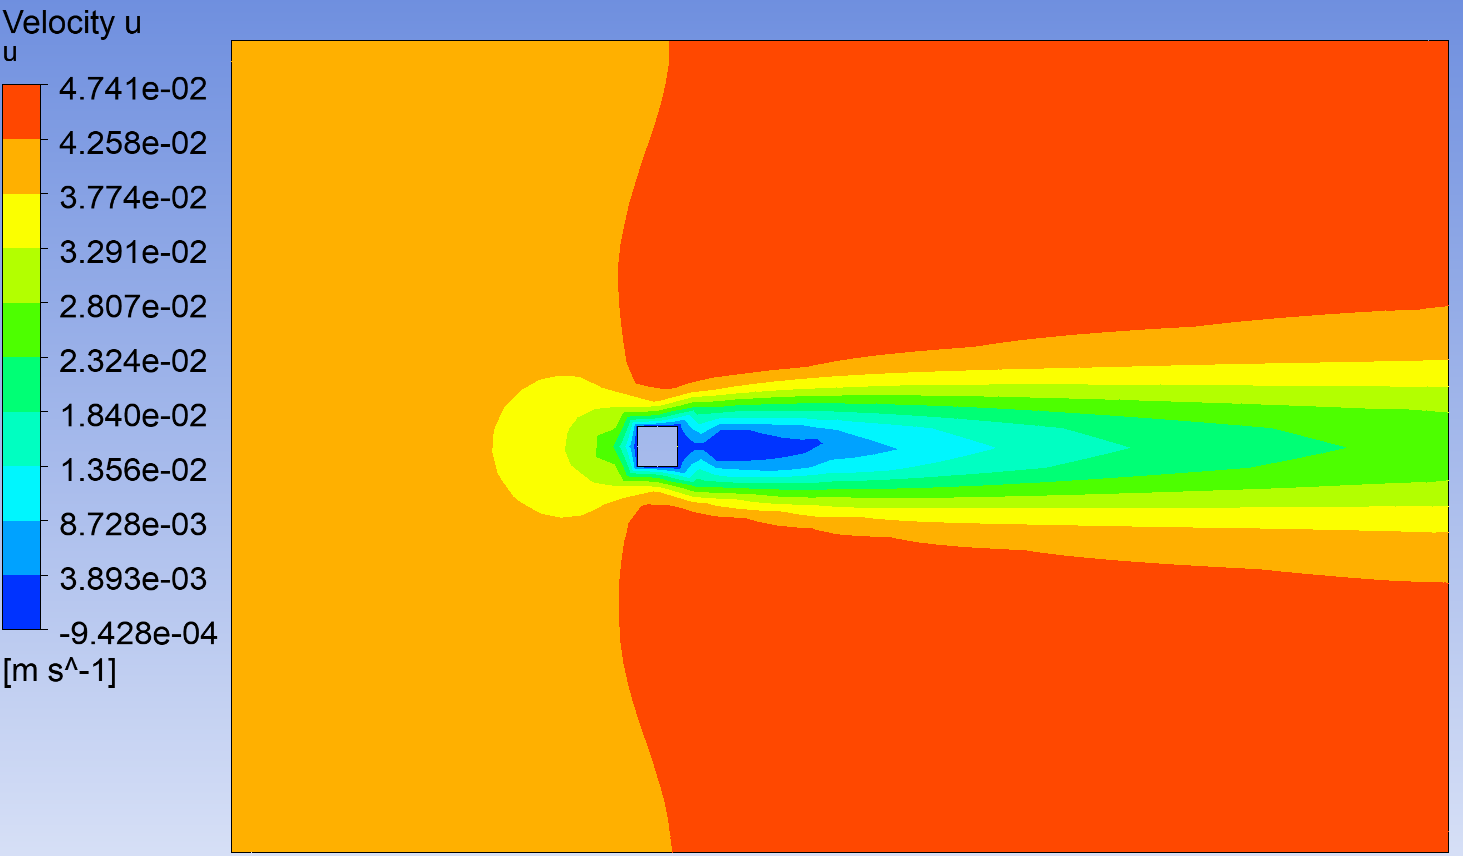
\includegraphics[width=\textwidth]{Questions/Figures/u velocity contour grid 1.png}
        \caption{Velocity Contour for Grid 1}
        \label{fig:velocity_contour_grid_1}
    \end{minipage}
    \begin{minipage}{0.45\textwidth}
        \centering
        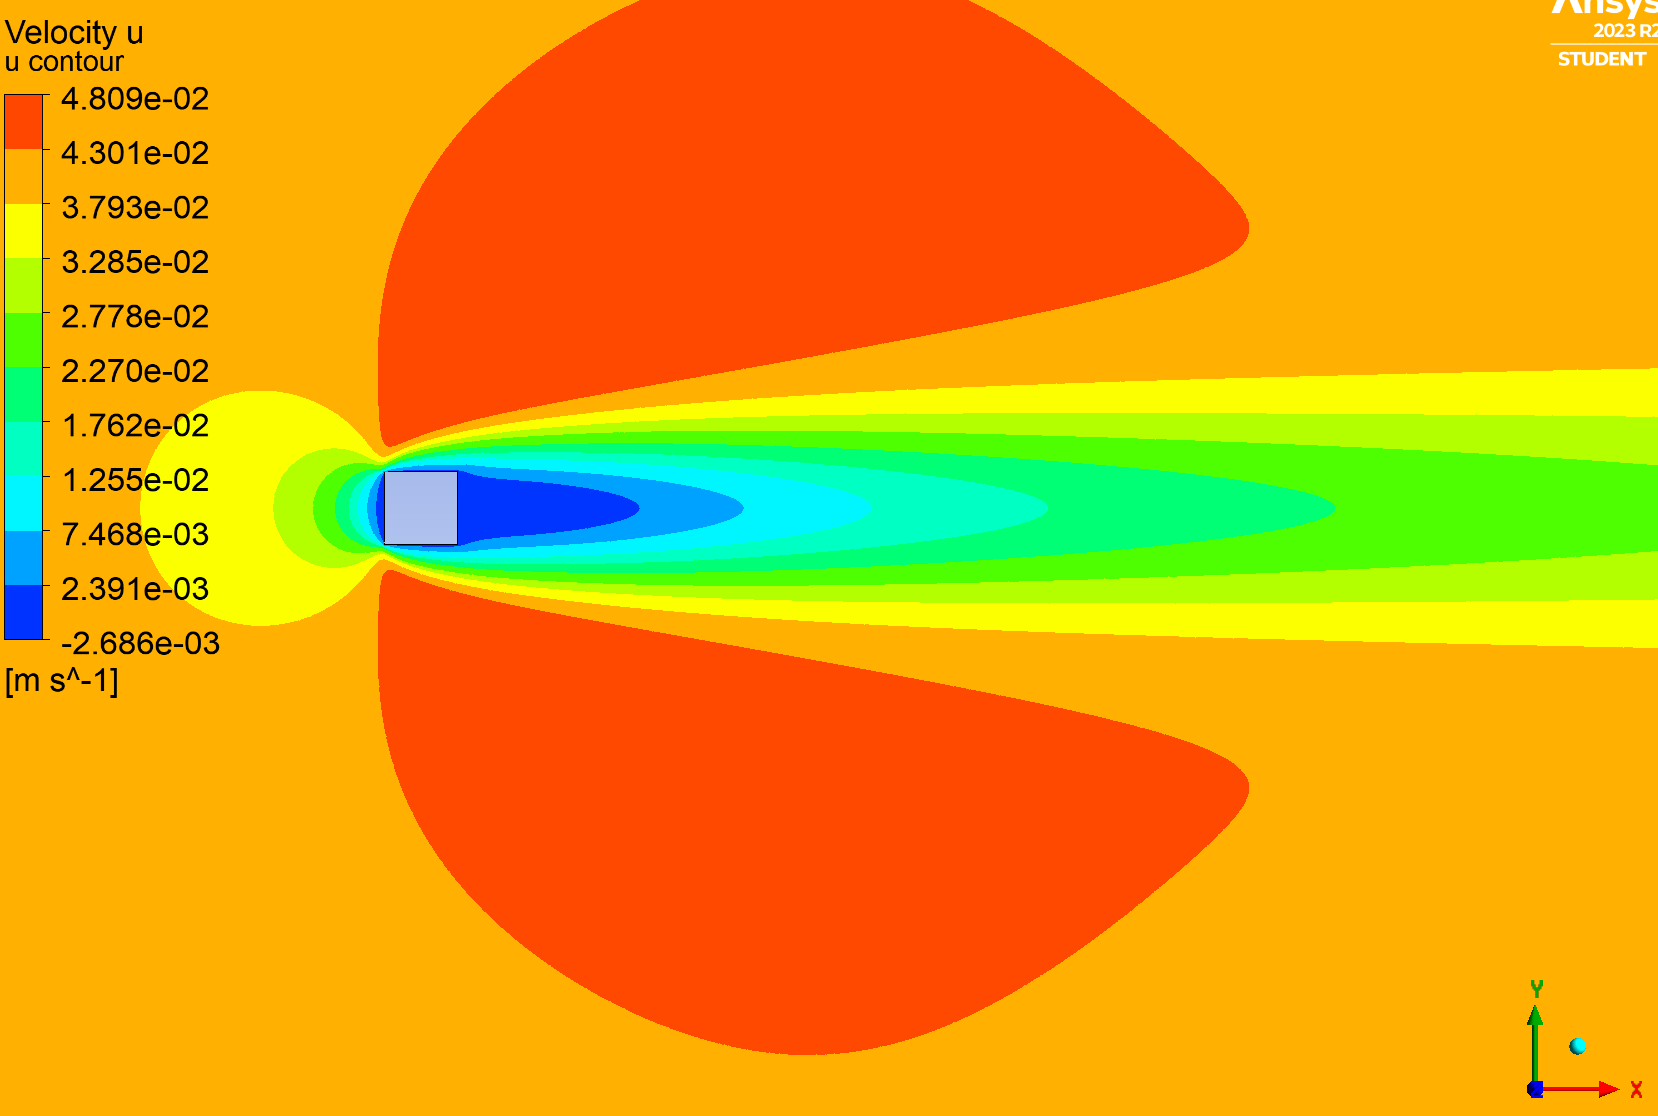
\includegraphics[width=\textwidth]{Questions/Figures/u velocity contour grid 5.png}
        \caption{Velocity Contour for Grid 5}
        \label{fig:velocity_contour_grid_5}
    \end{minipage}
\end{figure}
\begin{figure}[H]
    \centering
    \begin{minipage}{0.45\textwidth}
        \centering
        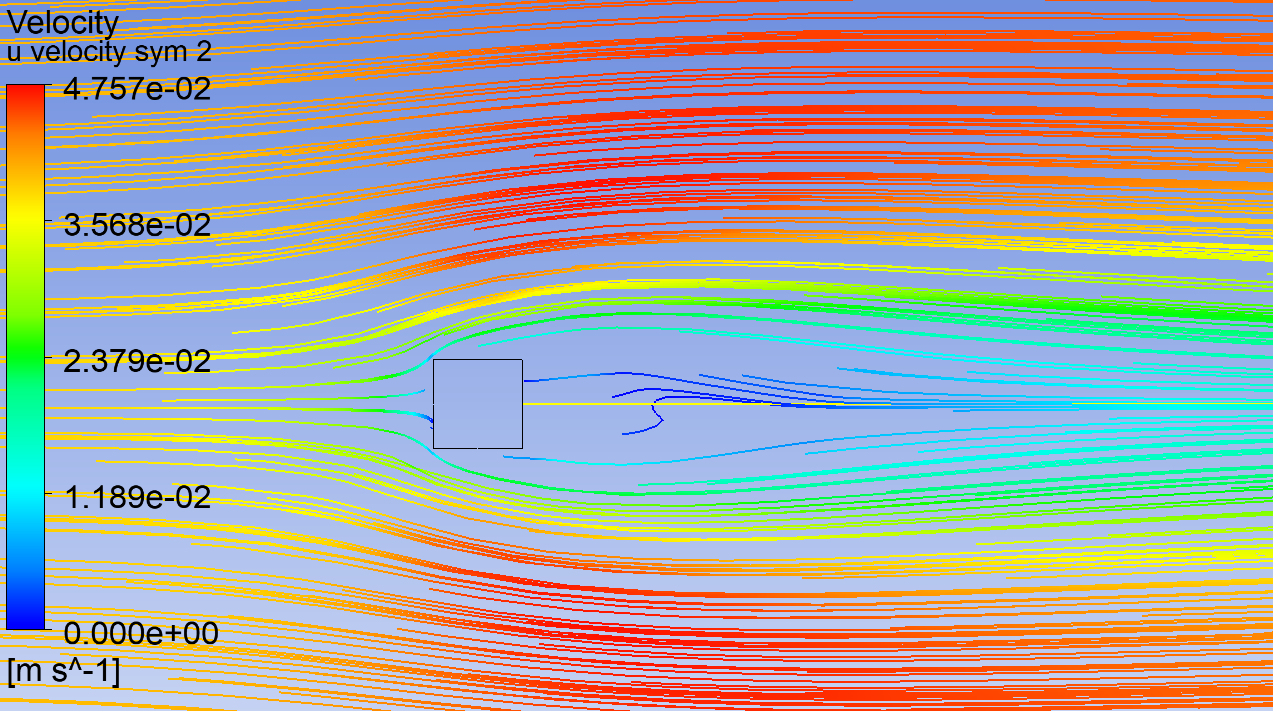
\includegraphics[width=\textwidth]{Questions/Figures/u velocity streamline grid 1.png}
        \caption{Streamlines for Grid 1}
        \label{fig:streamlines_grid_1}
    \end{minipage}
    \begin{minipage}{0.45\textwidth}
        \centering
        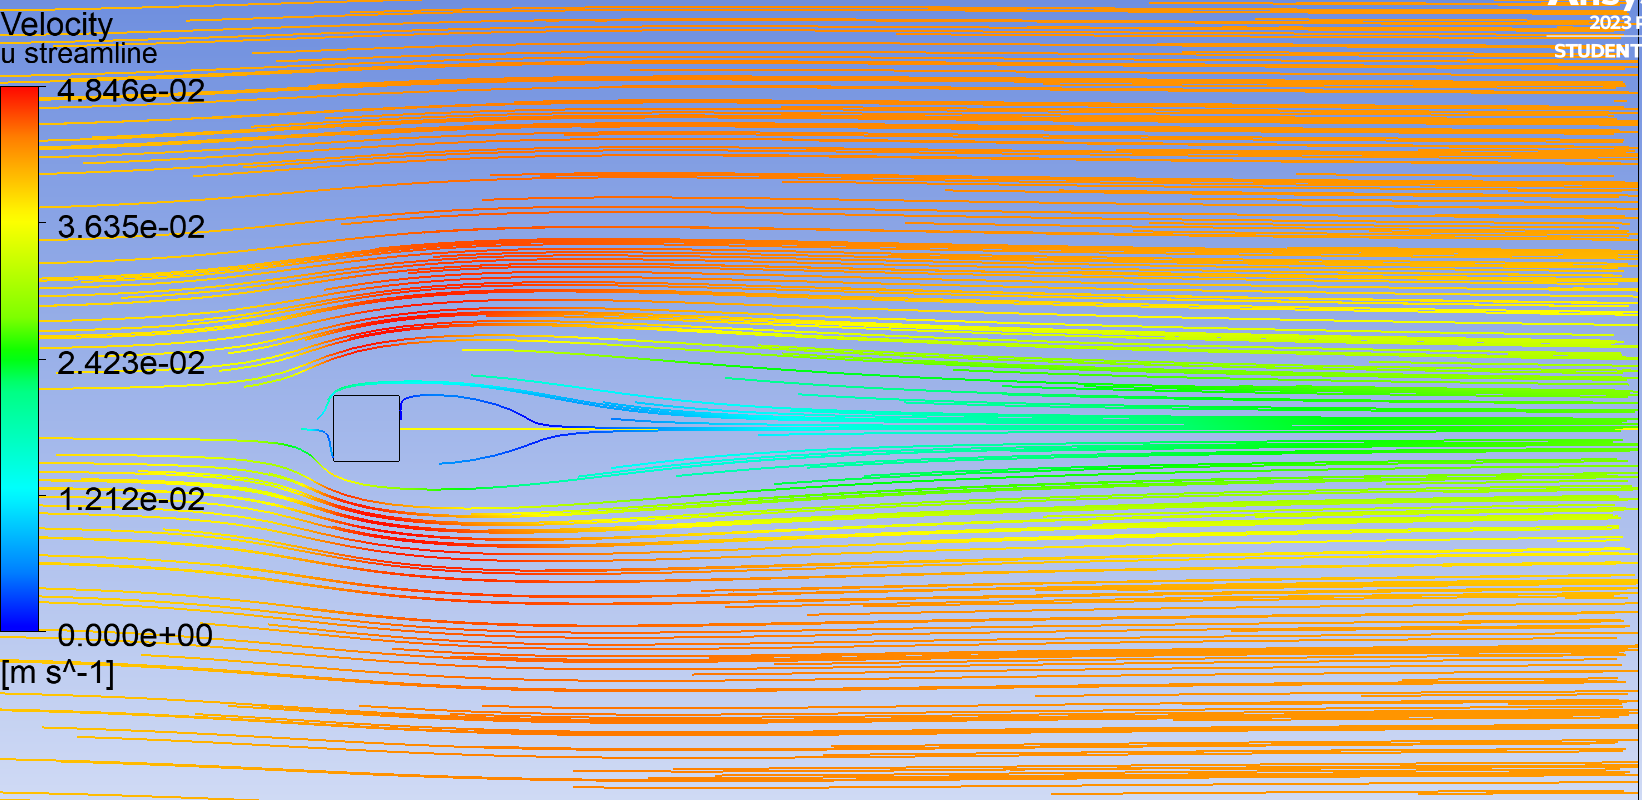
\includegraphics[width=\textwidth]{Questions/Figures/u velocity streamline grid 3.png}
        \caption{Streamlines for Grid 3}
        \label{fig:streamlines_grid_3}
    \end{minipage}
\end{figure}
\begin{figure}[H]
    \centering
    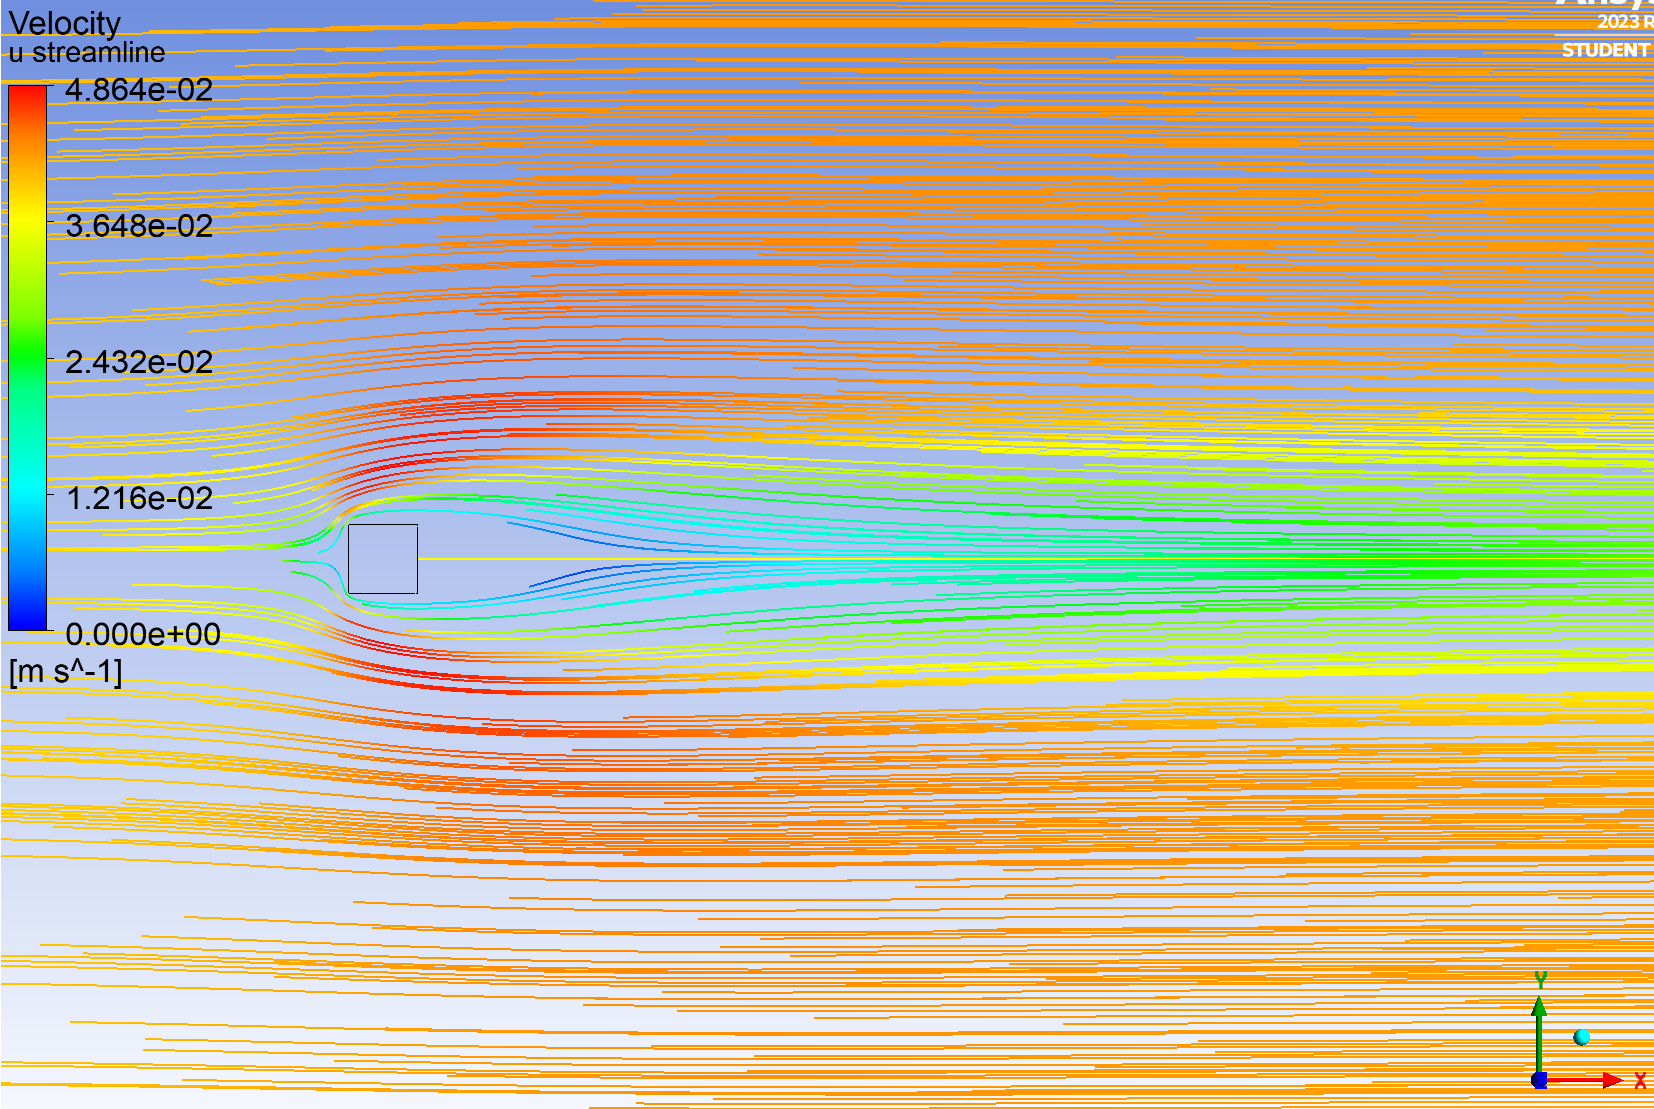
\includegraphics[width=0.45\textwidth]{Questions/Figures/u velocity streamline grid 5.png}
    \caption{Streamlines for Grid 5}
    \label{fig:streamlines_grid_5}
\end{figure}

\subsection{Drag Coefficient and Vortex Length}
\subsubsection{Vortex Length and Drag Coefficient}
The vortex length and drag coefficient are summarized in Table \ref{tab:vortex_length_drag_coefficient_summary}. 
\begin{table}[H]
    \centering
    \caption{Vortex Length and Drag Coefficient}
    \label{tab:vortex_length_drag_coefficient_summary}
    \begin{tabular}{cccc}
        \toprule
        Grid & Recirculation Length & Drag Coefficient \\
        & (m) & \\
        \midrule
        1 & 0.0115 & 3.1413 \\
        2 & 0.0181 & 2.7280 \\
        3 & 0.0186 & 2.5984 \\
        4 & 0.0183 & 2.5630 \\
        5 & 0.01801 & 2.5363 \\
        \bottomrule
    \end{tabular}
\end{table}
Sample calculations for grid 1 will be shown. The recirculation length is the distance between the two points ($x_1$, $x_2$) where the velocity is zero. Then
\begin{align*}
    L_r &= x_2 - x_1 \\
    &= 0.0234 - 0.0119 \\
    &= 0.0115 \text{ m}
\end{align*}
The drag coefficient is calculated as
\begin{align*}
    C_d &= \frac{2F_d}{\rho U_\infty^2 D} \\
    &= \frac{2 \times 2.51 \times 10^{-5}}{1.0 \times 0.04^2 \times 0.01} \\
    &= 3.1413
\end{align*}

\subsubsection{Recirculation Length on All Grids}
The combined plot of the velocity profile for all grids is shown in Figure \ref{fig:velocity_profile_all_grids}. Note, there is an issue with the coordinates of the line in grid 5 because the origin was defined slightly differently than grids 1-4 (by accident).

Grid 1 does not really have a recirculation length, while grid 2 shows some recirculation. In Grids 3-5, the concave shape develops and becomes steady around grid 4. Grid 3 seems to capture the details of grids 4 and 5 for $\tilde{}$ 16x fewer cells.

\begin{figure}[H]
    \centering
    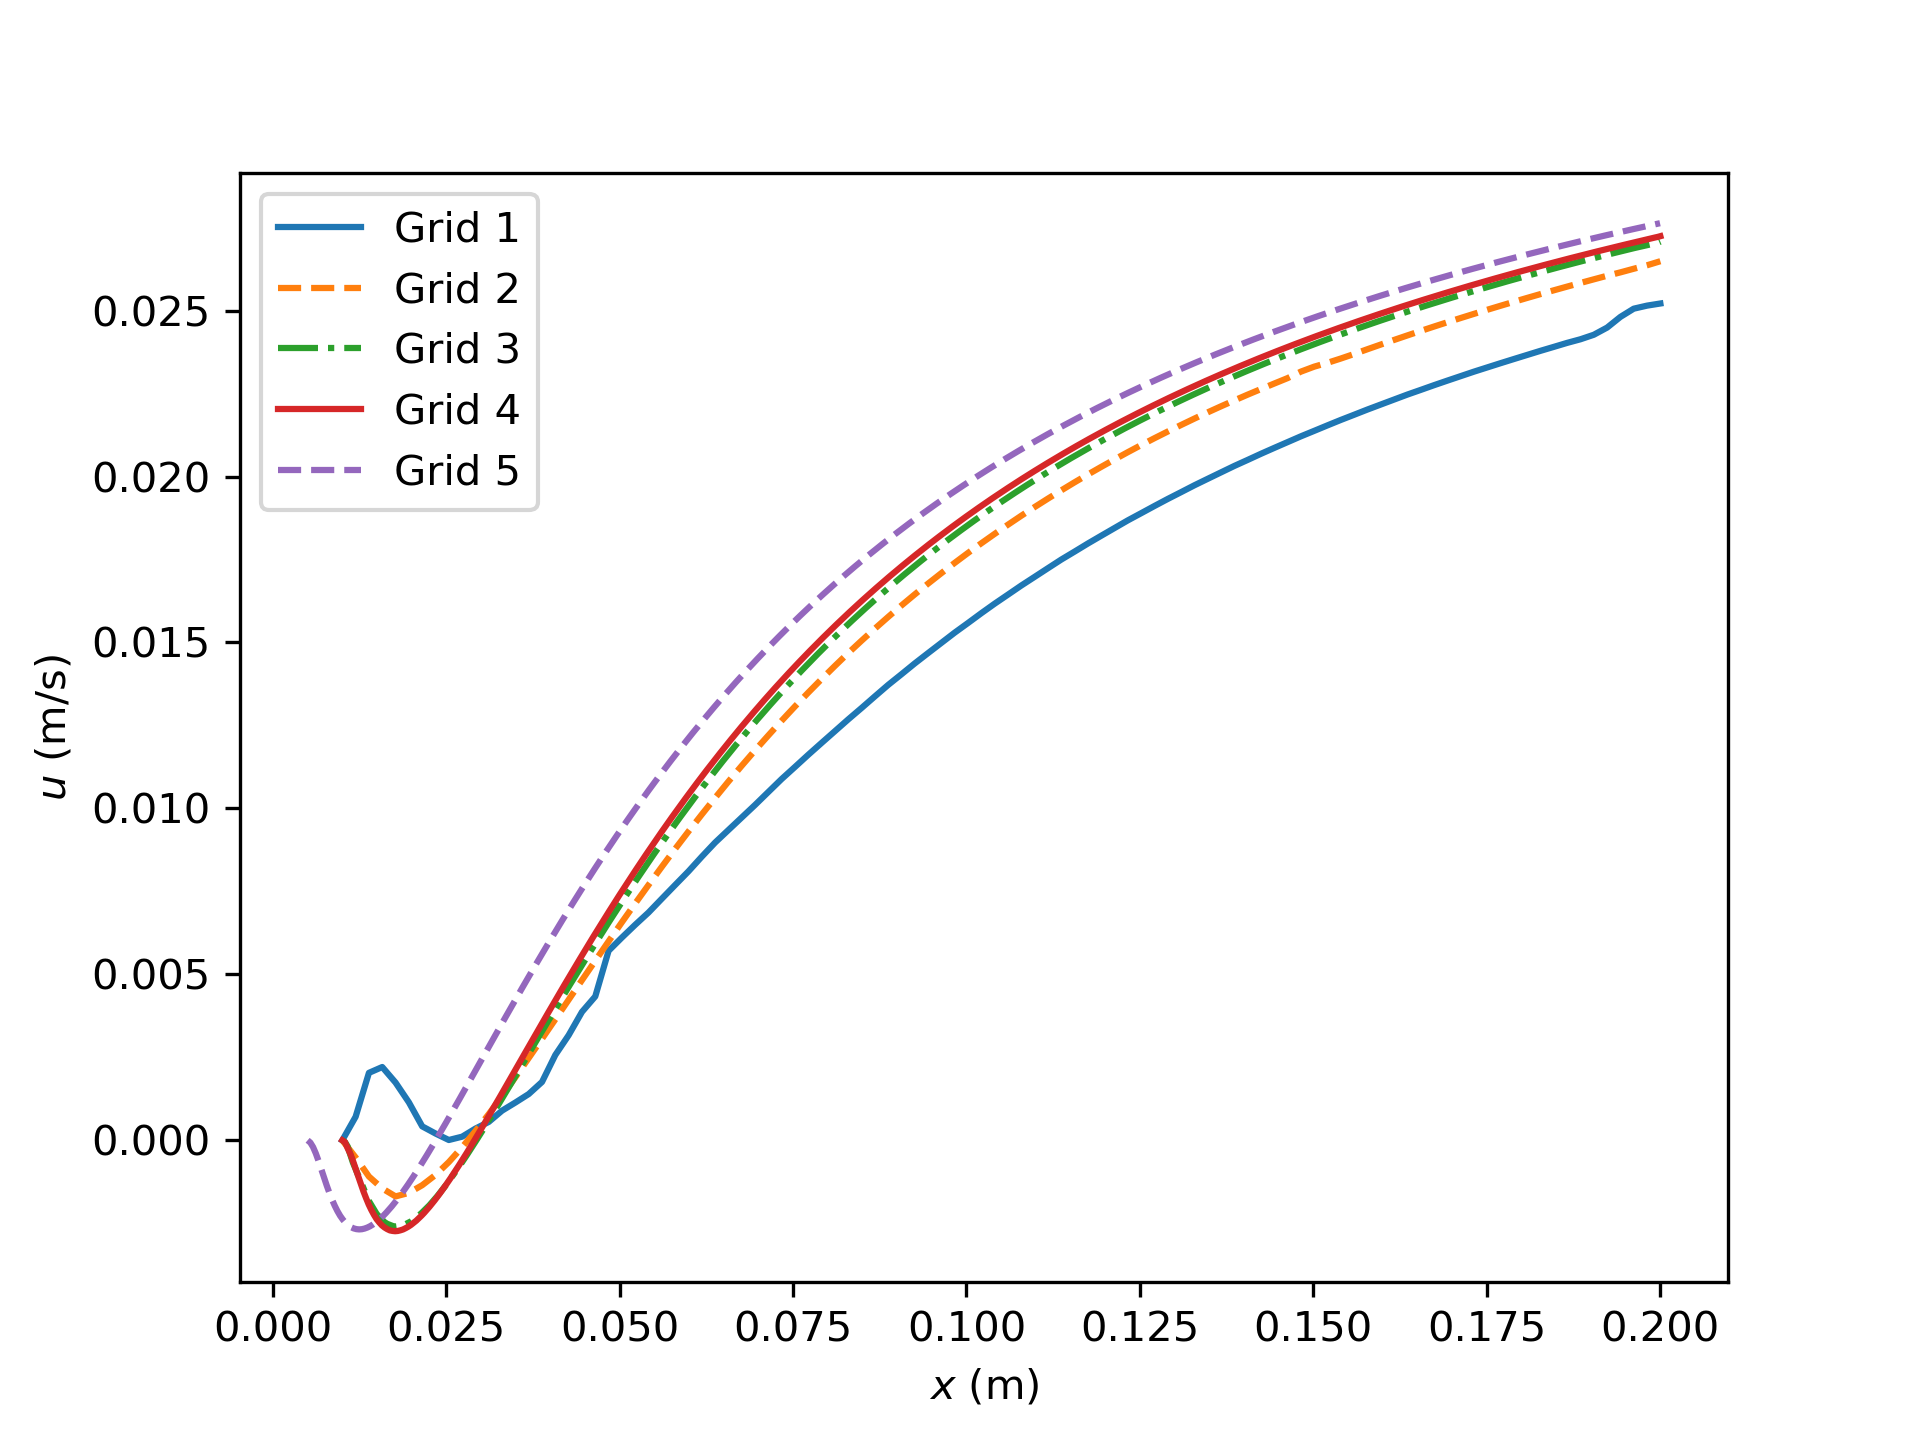
\includegraphics[width=0.5\textwidth]{Questions/Figures/recirc_combined.png}
    \caption{Velocity Profile for All Grids}
    \label{fig:velocity_profile_all_grids}
\end{figure}

\subsubsection{Mesh Independence}
\begin{figure}[H]
    \centering
    \begin{minipage}{0.45\textwidth}
        \centering
        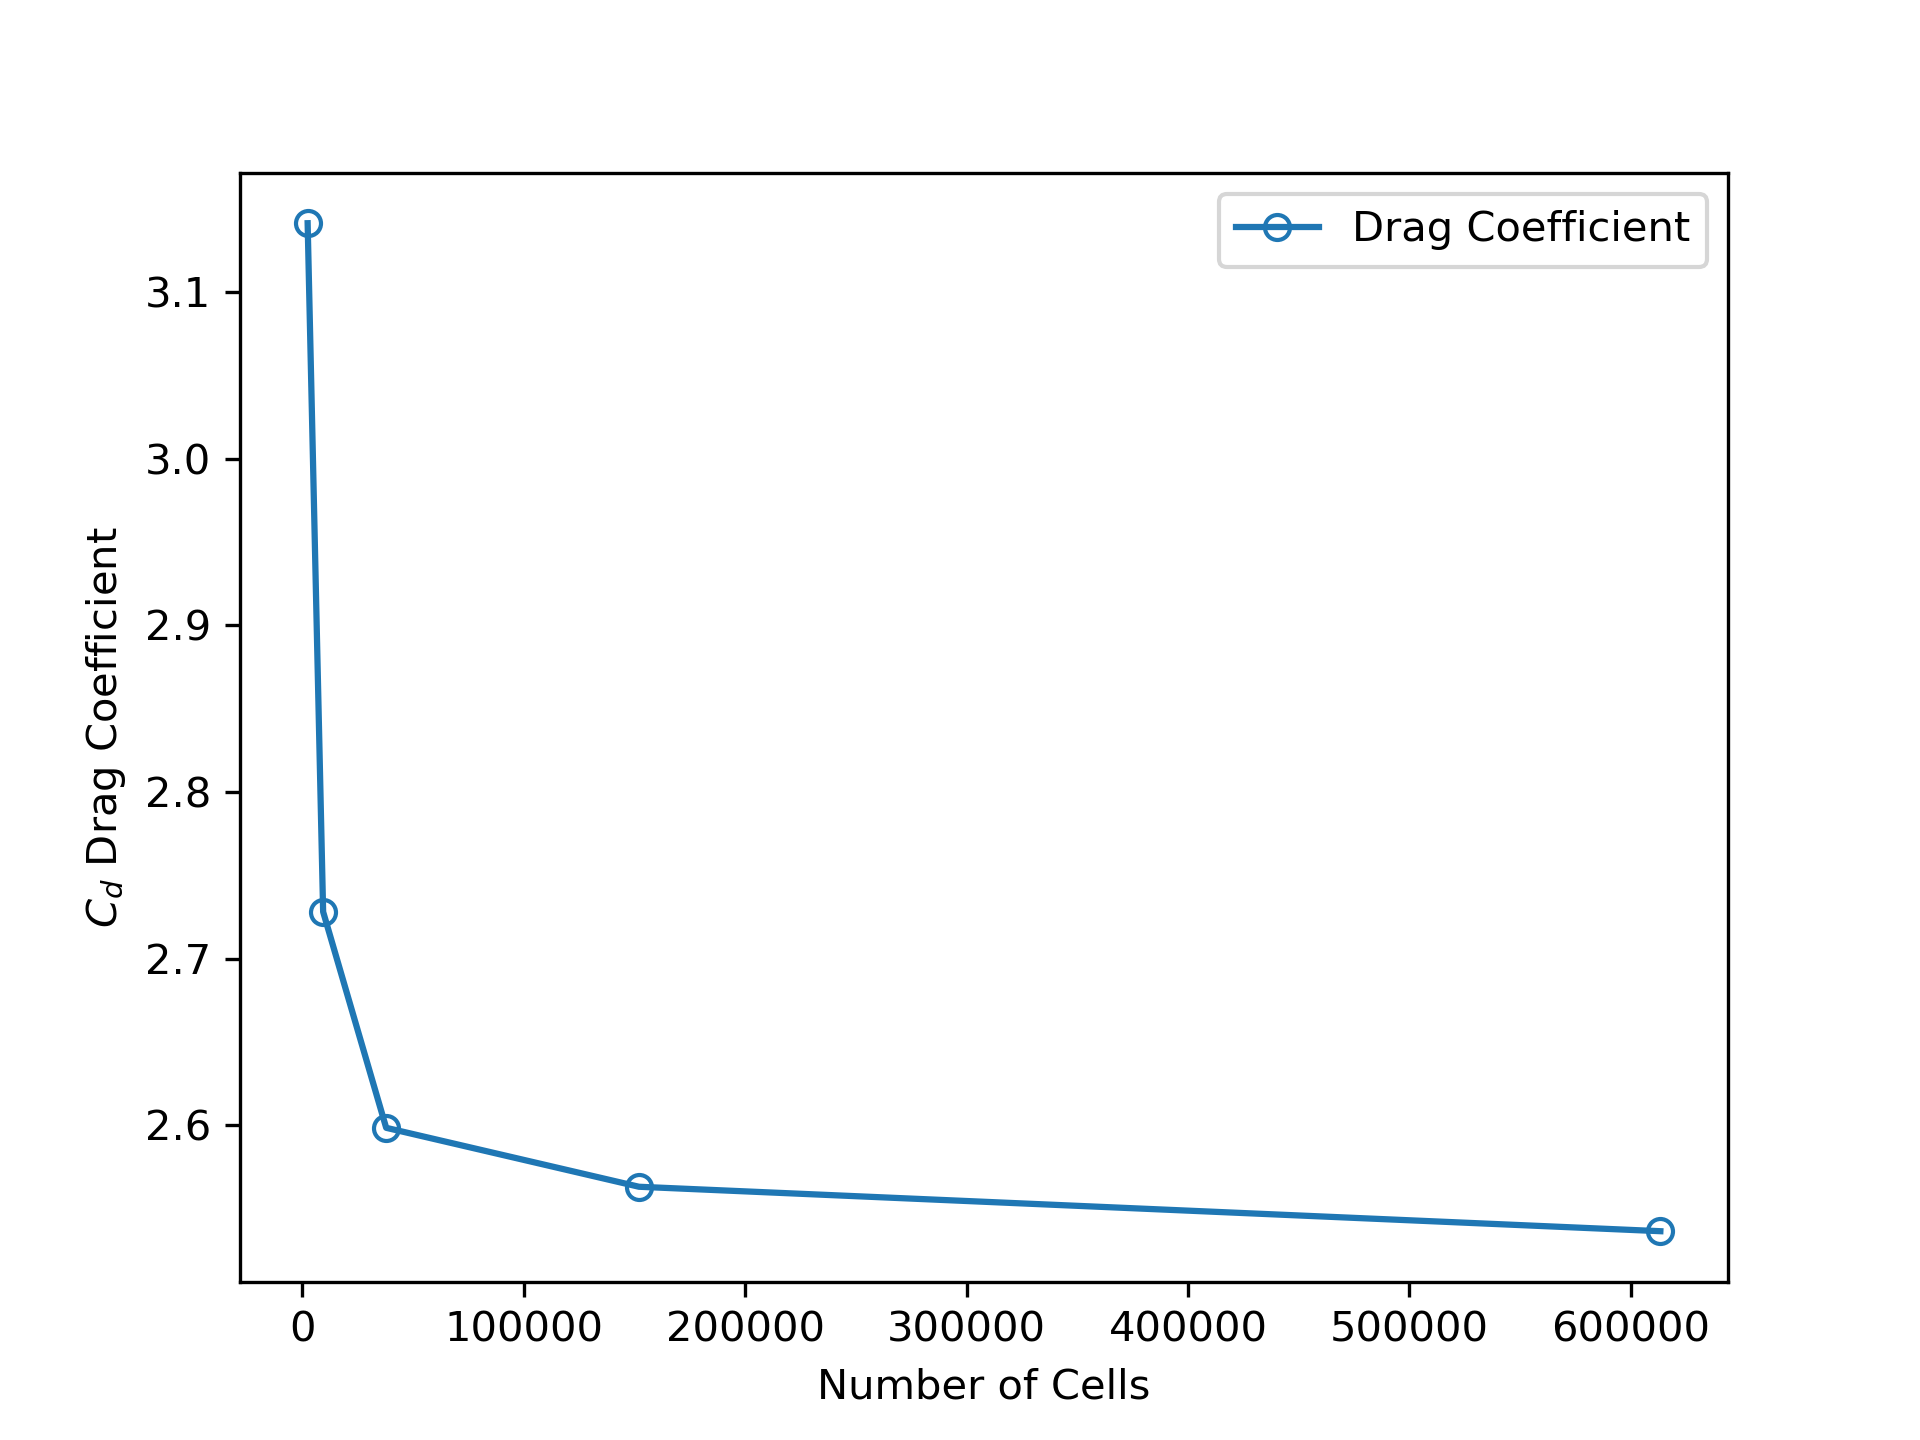
\includegraphics[width=\textwidth]{Questions/Figures/drag_coefficient_vs_cells.png}
        \caption{Drag Coefficient vs. Cells}
        \label{fig:drag_coefficient_vs_cells}
    \end{minipage}
    \begin{minipage}{0.45\textwidth}
        \centering
        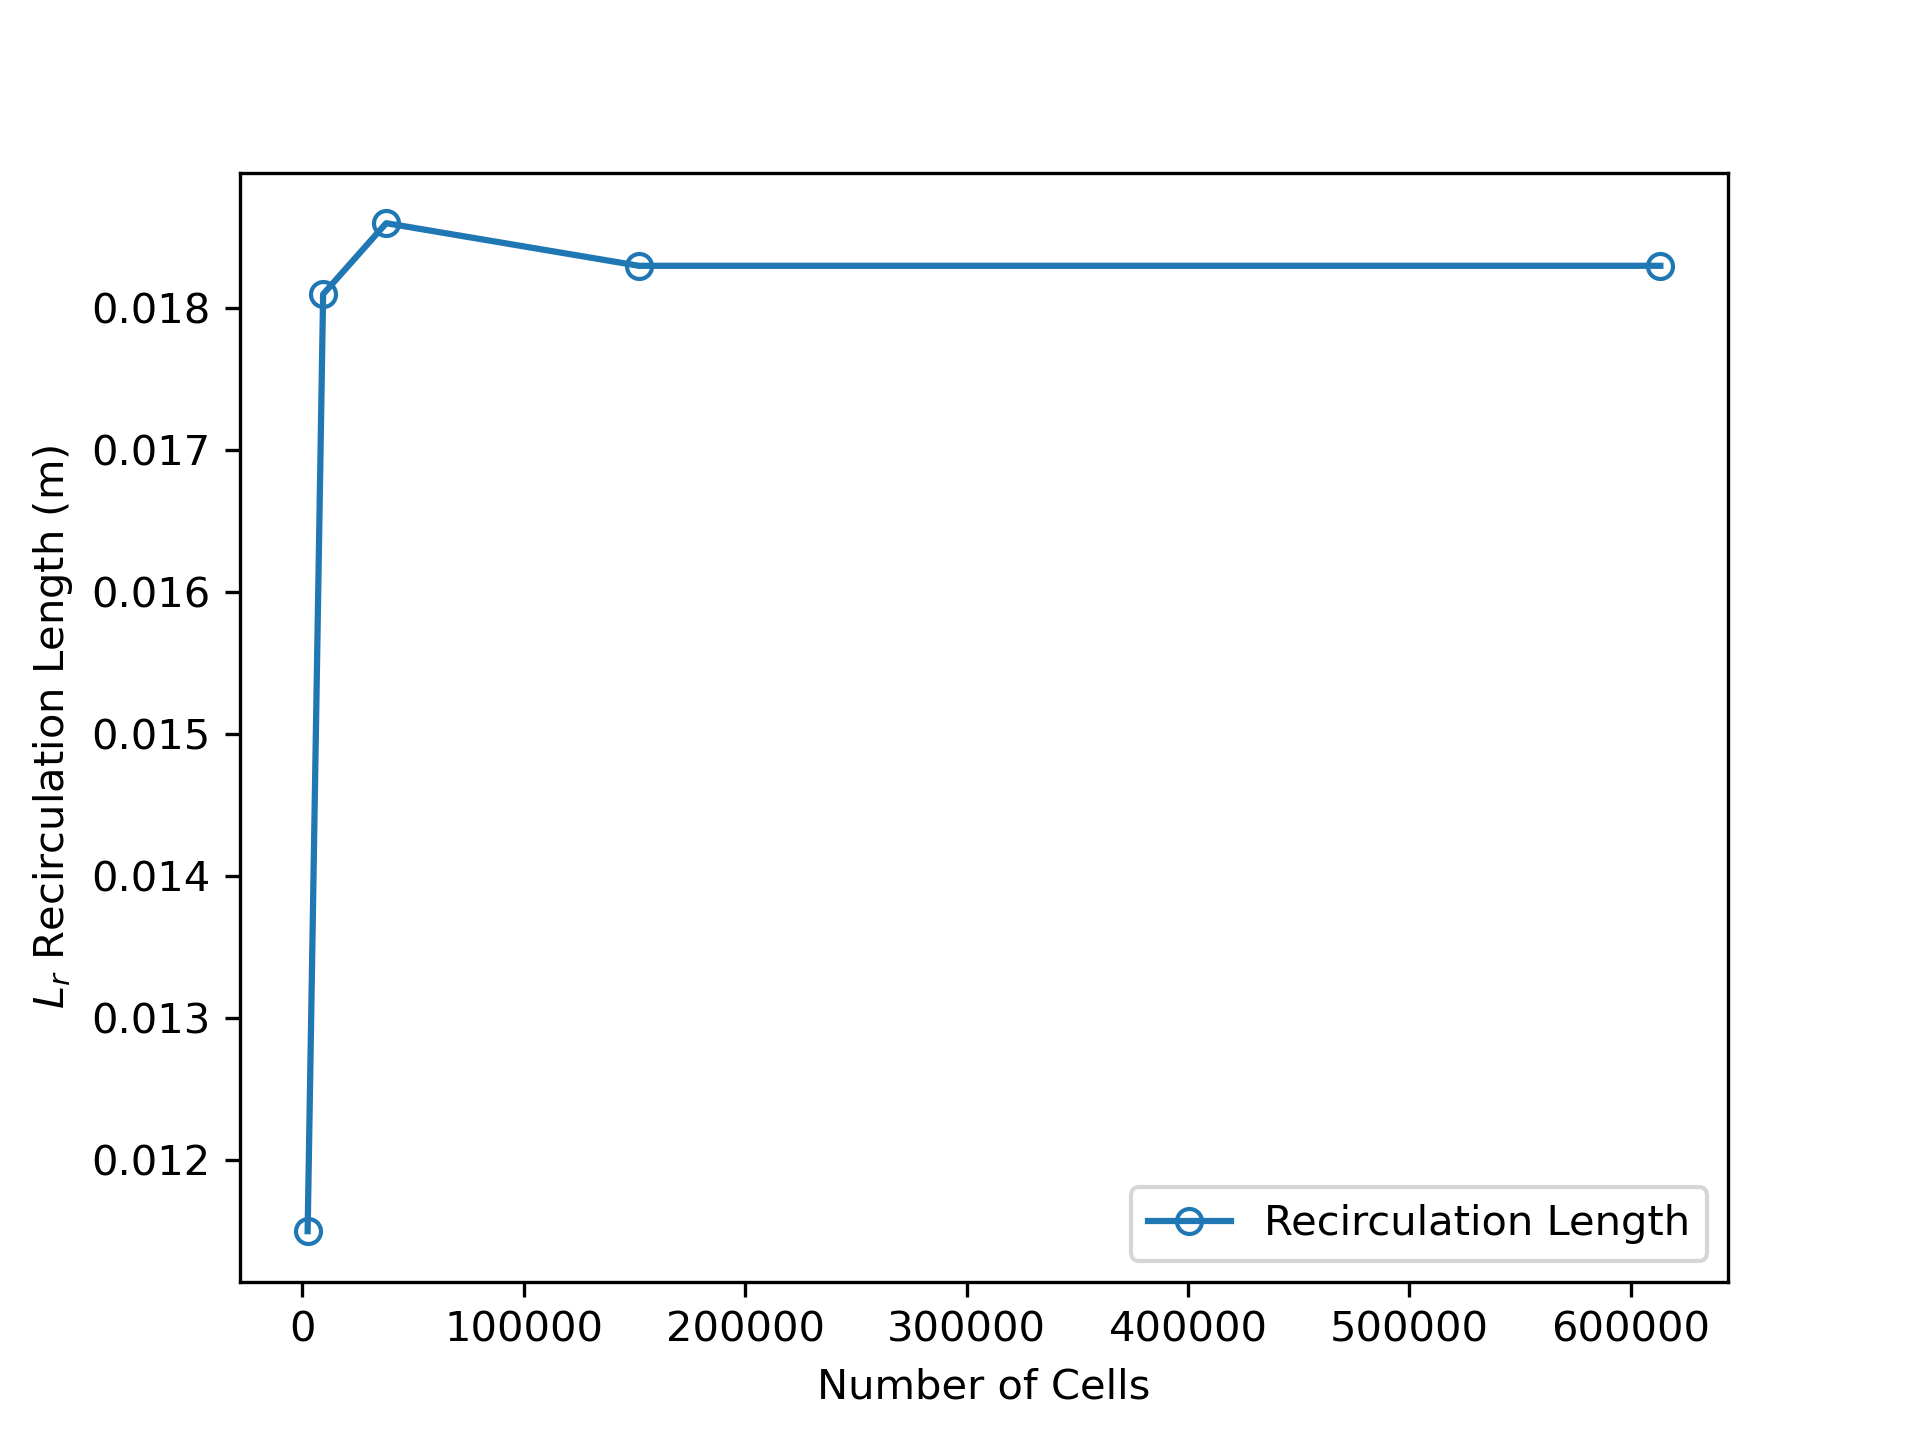
\includegraphics[width=\textwidth]{Questions/Figures/recirc_length_vs_cells.png}
        \caption{Recirculation Length vs. Cells}
        \label{fig:recirculation_length_vs_cells}
    \end{minipage}
\end{figure}
\begin{table}[H]
    \centering
    \caption{Error in Vortex Length and Drag Coefficient with Respect to Grid 5}
    \label{tab:error_vortex_length_drag_coefficient}
    \begin{tabular}{ccc}
        \toprule
        Grid & Vortex Length Error & Drag Coefficient Error \\
        & (\%) & (\%) \\
        \midrule
        1 & 36.15 & 23.85 \\
        2 & 0.50 & 7.56 \\
        3 & 3.28 & 2.45 \\
        4 & 1.61 & 1.05 \\
        5 & - & - \\
        \bottomrule
    \end{tabular}
\end{table}
The drag coefficient and recirculation length are plotted against the total number of cells in Figures \ref{fig:drag_coefficient_vs_cells} and \ref{fig:recirculation_length_vs_cells}. The drag coefficient and recirculation length become independent around mesh 3, with it's results being within 3\% of grid 5. The error in the vortex length and drag coefficient with respect to grid 5 is shown in Table \ref{tab:error_vortex_length_drag_coefficient}.

\subsection{Estimation of the Order of the Method}
First calculate the order of the method. The order is calculated as
\begin{align*}
    p &\approx \frac{\log\left(\frac{F_{\Delta x_4} - F_{\Delta x_3}}{F_{\Delta x_5} - F_{\Delta x_4}}\right)}{\log a } \\
    &= \frac{\log\left(\frac{2.05 - 2.08}{2.03 - 2.05}\right)}{\log 2} \\
    &= \boxed{0.407}
\end{align*}
This is not the expected value of 2. Grid independence has not been reached then.

The Richardson extrapolation is not valid since grid independence has not been reached. Regardless, calculating the Richardson extrapolation for grid 5 gives
\begin{align*}
    \epsilon &= \frac{C_{\Delta x_5} - C_{\Delta x_4}}{a^p - 1} \\
    &= -0.0818
\end{align*}
then,
\begin{align*}
    C_{\text{exact}} &\approx C_{\Delta x_5} + \epsilon \\
    &= 2.5363 - 0.0818 \\
    &= 2.4546
\end{align*}
The error in the drag coefficient against the element size is shown in Figure \ref{fig:richardson_error_vs_element_size}. 
\begin{figure}[H]
    \centering
    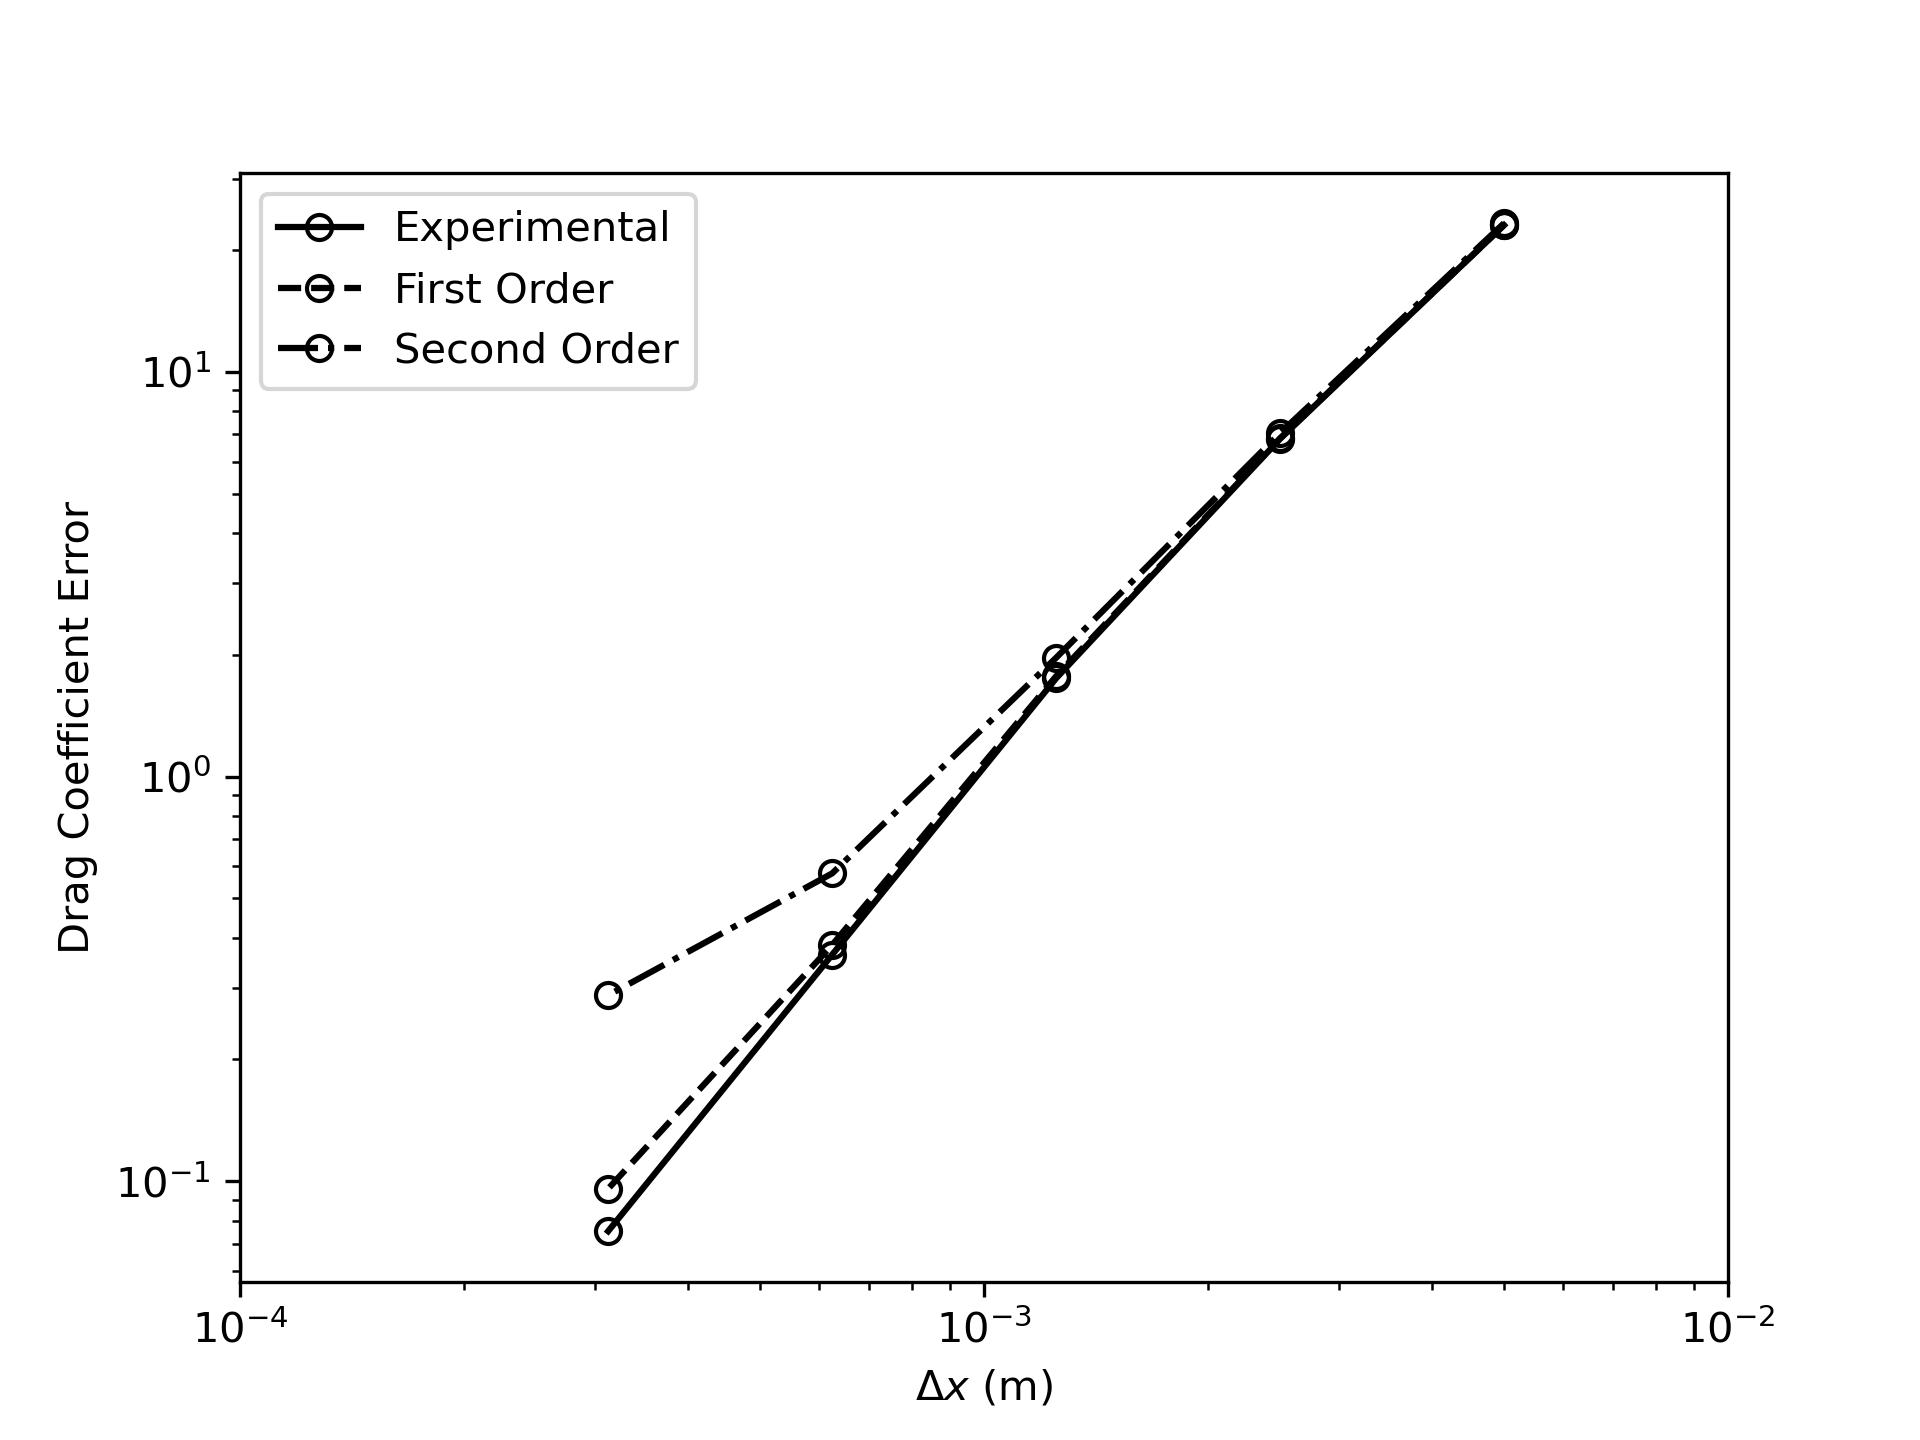
\includegraphics[width=0.5\textwidth]{Questions/Figures/richardson_error_vs_element_size.png}
    \caption{Error in Drag Coefficient vs. Element Size}
    \label{fig:richardson_error_vs_element_size}
\end{figure}
The error graph is higher than the first and second order error lines. This was expected since $p \approx 0.407$, which suggests low order convergence.

It would be expected that $1 < p_{\text{exp}} < 2$ since a second order scheme was used (not exactly 2 due to meshing impurities). For unknown reasons, this was not achieved. Further work would be needed to determine why the expected order was not achieved.

\subsection{Validation of the Results}
From another study, the drag coefficient was found to be  1.5657 \cite{paper} at a Reynolds number of 60. The drag coefficient was found to be 2.5363 at a Reynolds number of 20, which is the same order of magnitude. The relative error is then
\begin{align*}
    \text{Relative Error} &= \frac{2.5363 - 1.5657}{1.5657} \times 100\% \\
    &= \boxed{61.99\%}
\end{align*}